\section{Użycie Kaskad w celu realizacji Tricku (Maciej Plewka)}

W tym rozdziale opisany zostanie sposób użycia kaskady do zrealizowania dwóch wariantów sztuczki. Pierwszy to ten w którym wklejana jest karta w miejsce odnalezienia czoła, w drugim przypadku zamieszczamy ją w miejsce wyznaczonego obiektu. Opisany także będą sposoby dzięki którym osiągnięto optymalną skuteczność.

\subsection{Detekcja Czoła}

W celu detekcji czoła wykorzystano kaskady zapisane w plikach w plikach z rozszerzeniem xml, które są dołączone razem z biblioteką openCV. Wykorzystano plik kaskadowy pliki lbpcascade\_frontalface.xml oraz haarcascade\_lefteye\_2splits.xml.
Pierwszy z nich opisuje klasyfikatory służąca do rozpoznawania przodu twarzy, drugi 
Teoretycznie służy do detekcji lewego oka które jest otwarte. Kaskada służąca do rozpoznawania lewego oka w praktyce jest wstanie skutecznie rozpoznać także prawe oko a także jeśli chcemy wykorzystać ją do detekcji obu oczu radzi sobie lepiej niż kaskada odpowiedzialna za prawe oko. W naszej aplikacji miejsce czoła zostaje wyznaczone na podstawie informacji na temat położenia twarzy oraz oczu. Wykrywanie oczu zostaje uruchomione w momencie rozpoznania twarzy, gdyż wiadomym jest, że do poprawnego wykrycia oczu muszą się one znajdować w twarzy. 
Następnie, jeśli udało się nam odnaleźć w zdjęciu twarz a w niej parę oczu uznajemy że detekcja przebiegła poprawnie. Zwrócone obiekty są typu Rect jest to typ z biblioteki openCV. W tym momencie wyznaczamy matematycznie domniemane miejsce czoła na podstawie położenia na zdjęciu twarzy oraz oczu. Lecz zanim określimy dokładne miejsce czoła należy określić które oko znajduje się po lewej.
Za lewy dolny punkt czoła przyjmiemy lewy górny punkt oka znajdującego się po lewej stronie, natomiast prawy dolny punkt jest równy co do wartości prawemu górnemu rogowi oka prawego. Różnica tych wartości jest zatem szerokością czoła. Wysokość czoła jest to szerokość czoła podzielona przez 2 albo jeśli wyznaczona w ten sposób wartość nie znajduje się w obrębie twarzy za wysokość przyjmujemy różnice między wyznaczonymi dolnymi punktami czoła a współrzędną y prostokąta znajdującego się w twarzy.


\subsection{Detekcja Karty}

W odróżnieniu od detekcji czoła znalezienie karty ogranicza się do zawołania metody detectmultiscale na wcześniej załadowanej kaskadzie. Po otrzymaniu informacji na temat odnalezionych obiektów analizuje się ich liczbę. Przyjęto by detekcja oceniana była jako poprawna musi być odnaleziony dokładnie jeden element, ponieważ sztuczka będzie wykonywana jednej osobie na raz, osoba ta będzie trzymać jedną kartę. W przypadku w którym rozpoznany będzie więcej niż jeden obiekt lub nie odnaleziony będzie ani jeden zostanie zwrócony komunikat o potrzebie ponownego wykonania zdjęcia.

\subsection{Dobór parametrów detekcji}

Parametry które mają wpływ na skuteczność klasyfikatora podczas detekcji oraz sprawiają, że cały proces trwa dłużej są:
\begin{itemize}
    \item -minNeighbors
    \item -scaleFactor
\end{itemize}

Parametr scaleFactor determinuje różnice między wielkościami ramki, w której szukany jest obiekt, podczas kolejnych iteracji algorytmu. Mała wartość tego parametru ogranicza przypadek pominięcia szukanego wzorca. Jeśli jednak badanych jest więcej obszarów rośnie nie tylko możliwych do odkrycia obiektów ale jest to także liczba miejsc w których może zostać podjęta błędna decyzja. Dodatkowo duża liczba miejsc do przeanalizowania znacząco wydłuża czas działania detekcji. Duża wartość tego współczynnika może spowodować przeoczenie obiektu.


\begin{figure}[H]
    \centering
        \begin{subfigure}{0.32\textwidth}
        \centering
        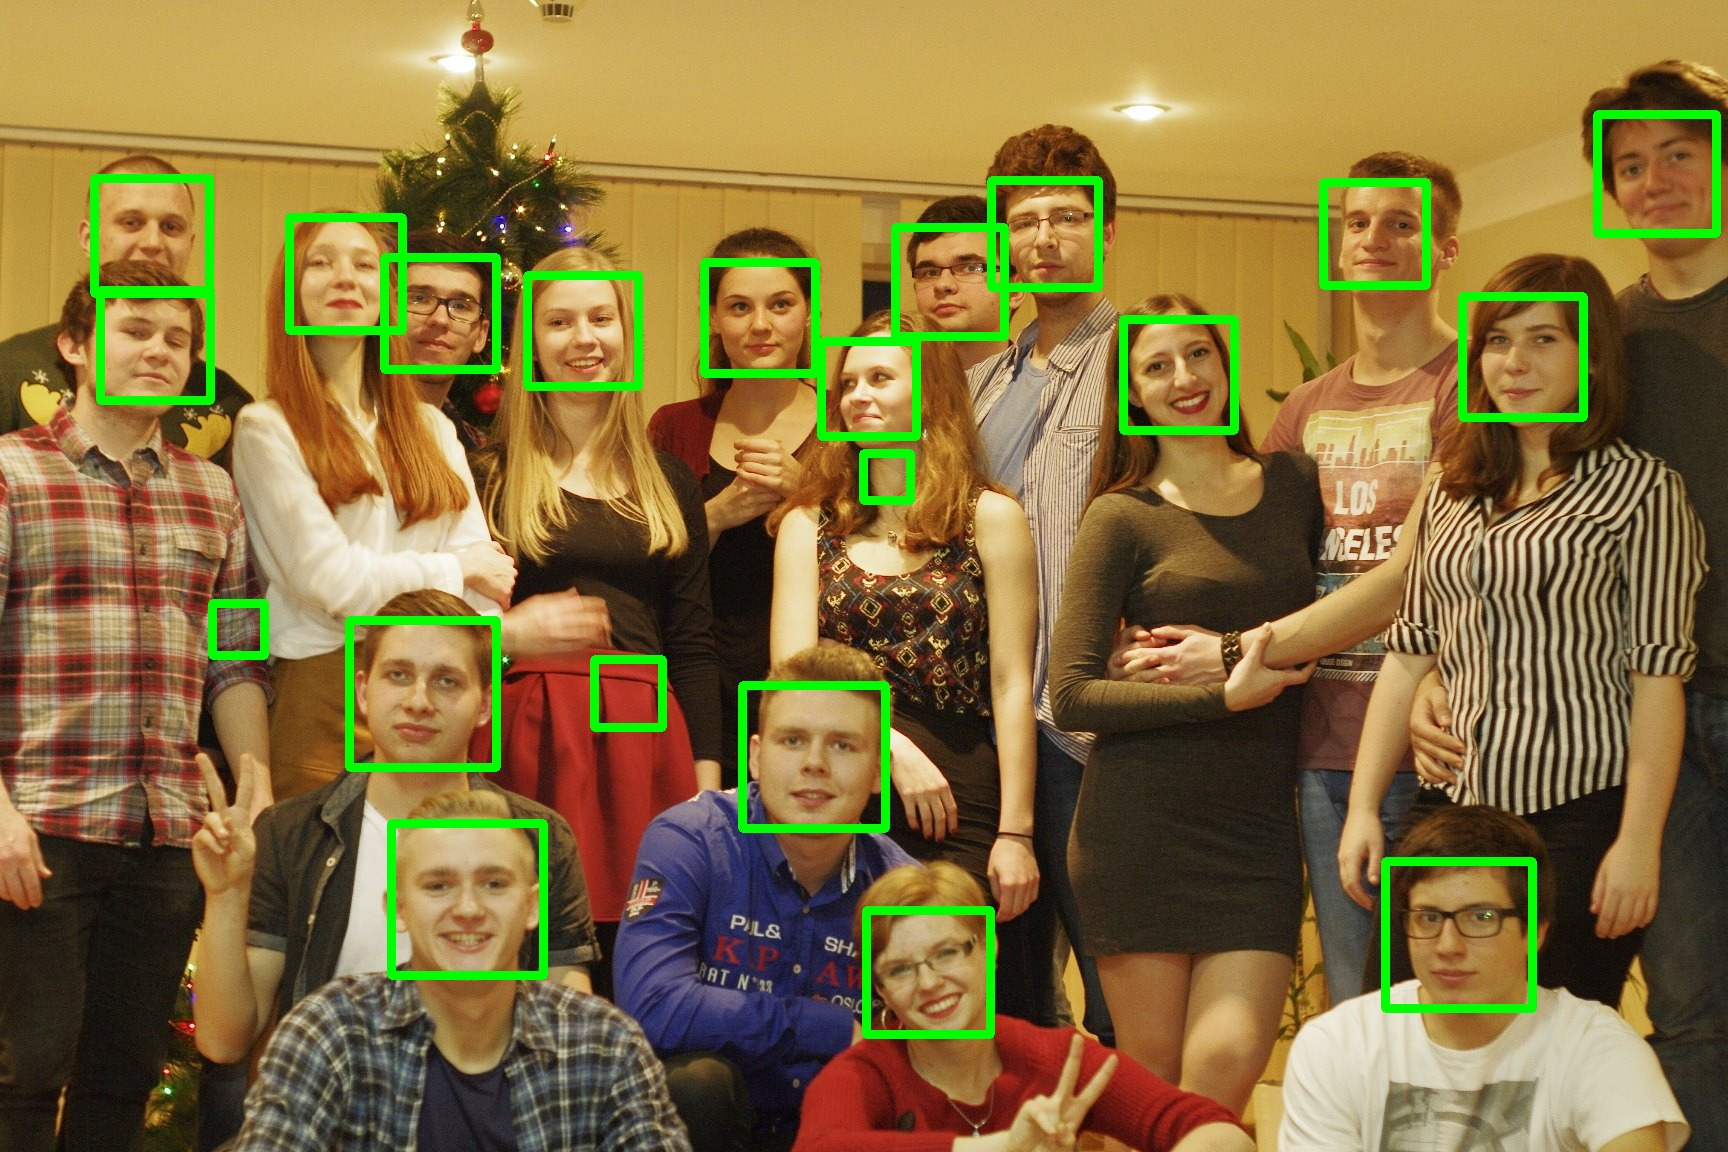
\includegraphics[width=\linewidth]{imgs/twarze11.jpg}
        \caption{skala 1.1}
        \label{fig:twarzSkala11}
    \end{subfigure}\hfill
    \begin{subfigure}{0.32\textwidth}
        \centering
        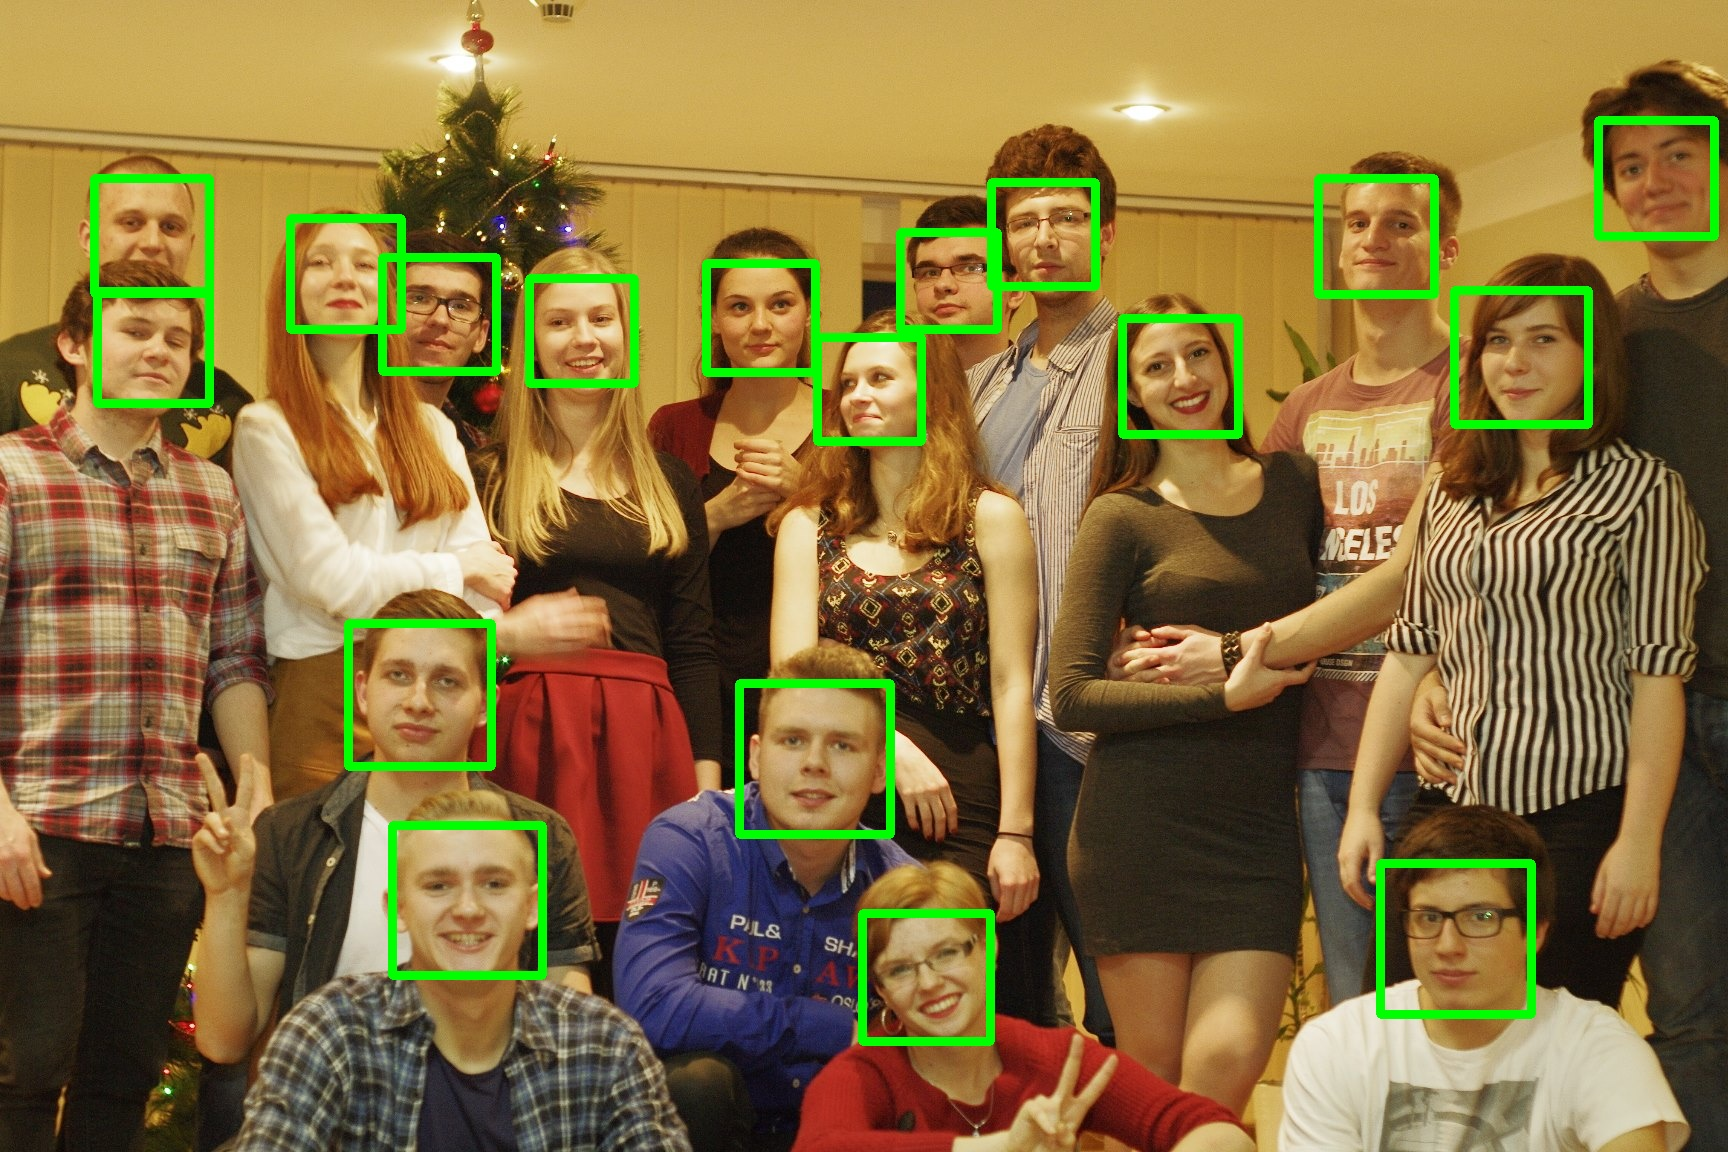
\includegraphics[width=\linewidth]{imgs/twarze13.jpg}
        \caption{skala 1.3}
        \label{fig:twarzSkala13}
    \end{subfigure}\hfill
    \begin{subfigure}{0.32\textwidth}
        \centering
        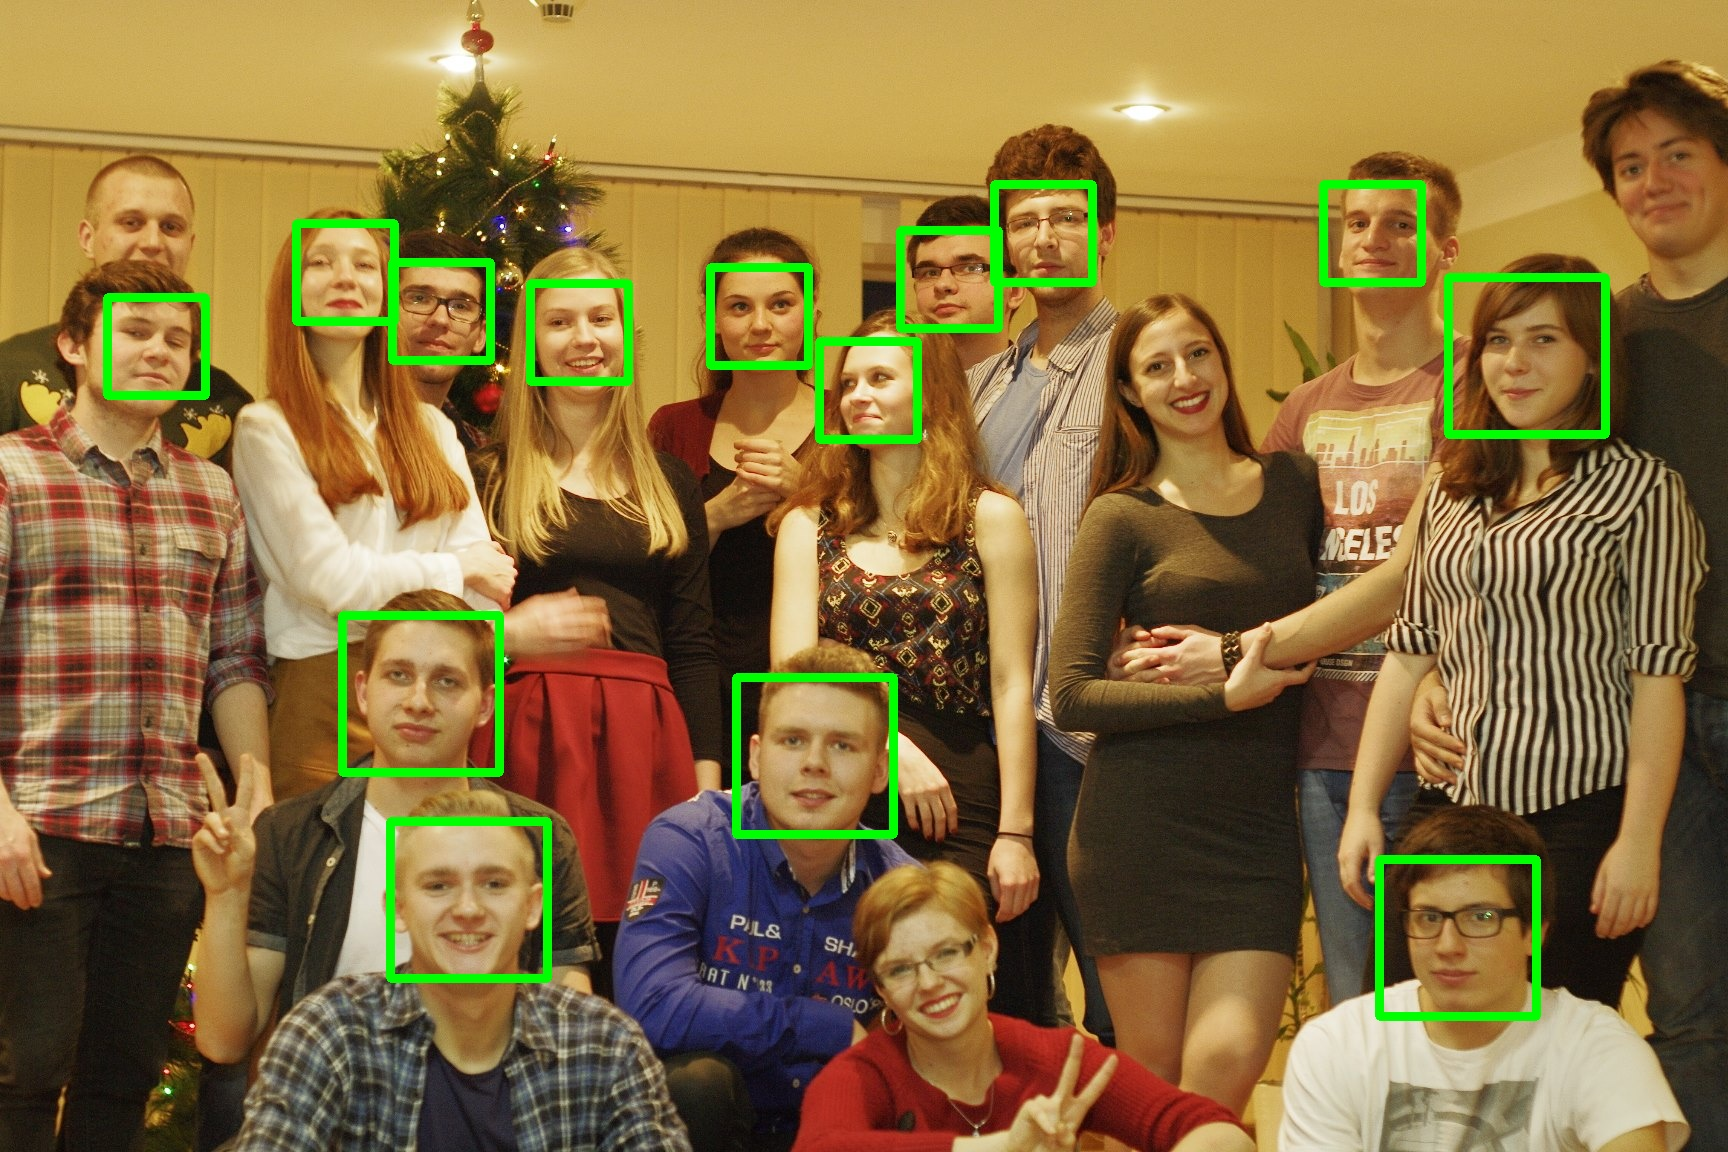
\includegraphics[width=\linewidth]{imgs/twarze16.jpg}
        \caption{skala 1.6}
        \label{fig:twarzSkala16}
    \end{subfigure}
    \caption{Detekcja twarzy dla różnych wartości scaleFactor}
    \label{twarzee}
\end{figure}

\begin{figure}[H]
    \centering
        \begin{subfigure}{0.32\textwidth}
        \centering
        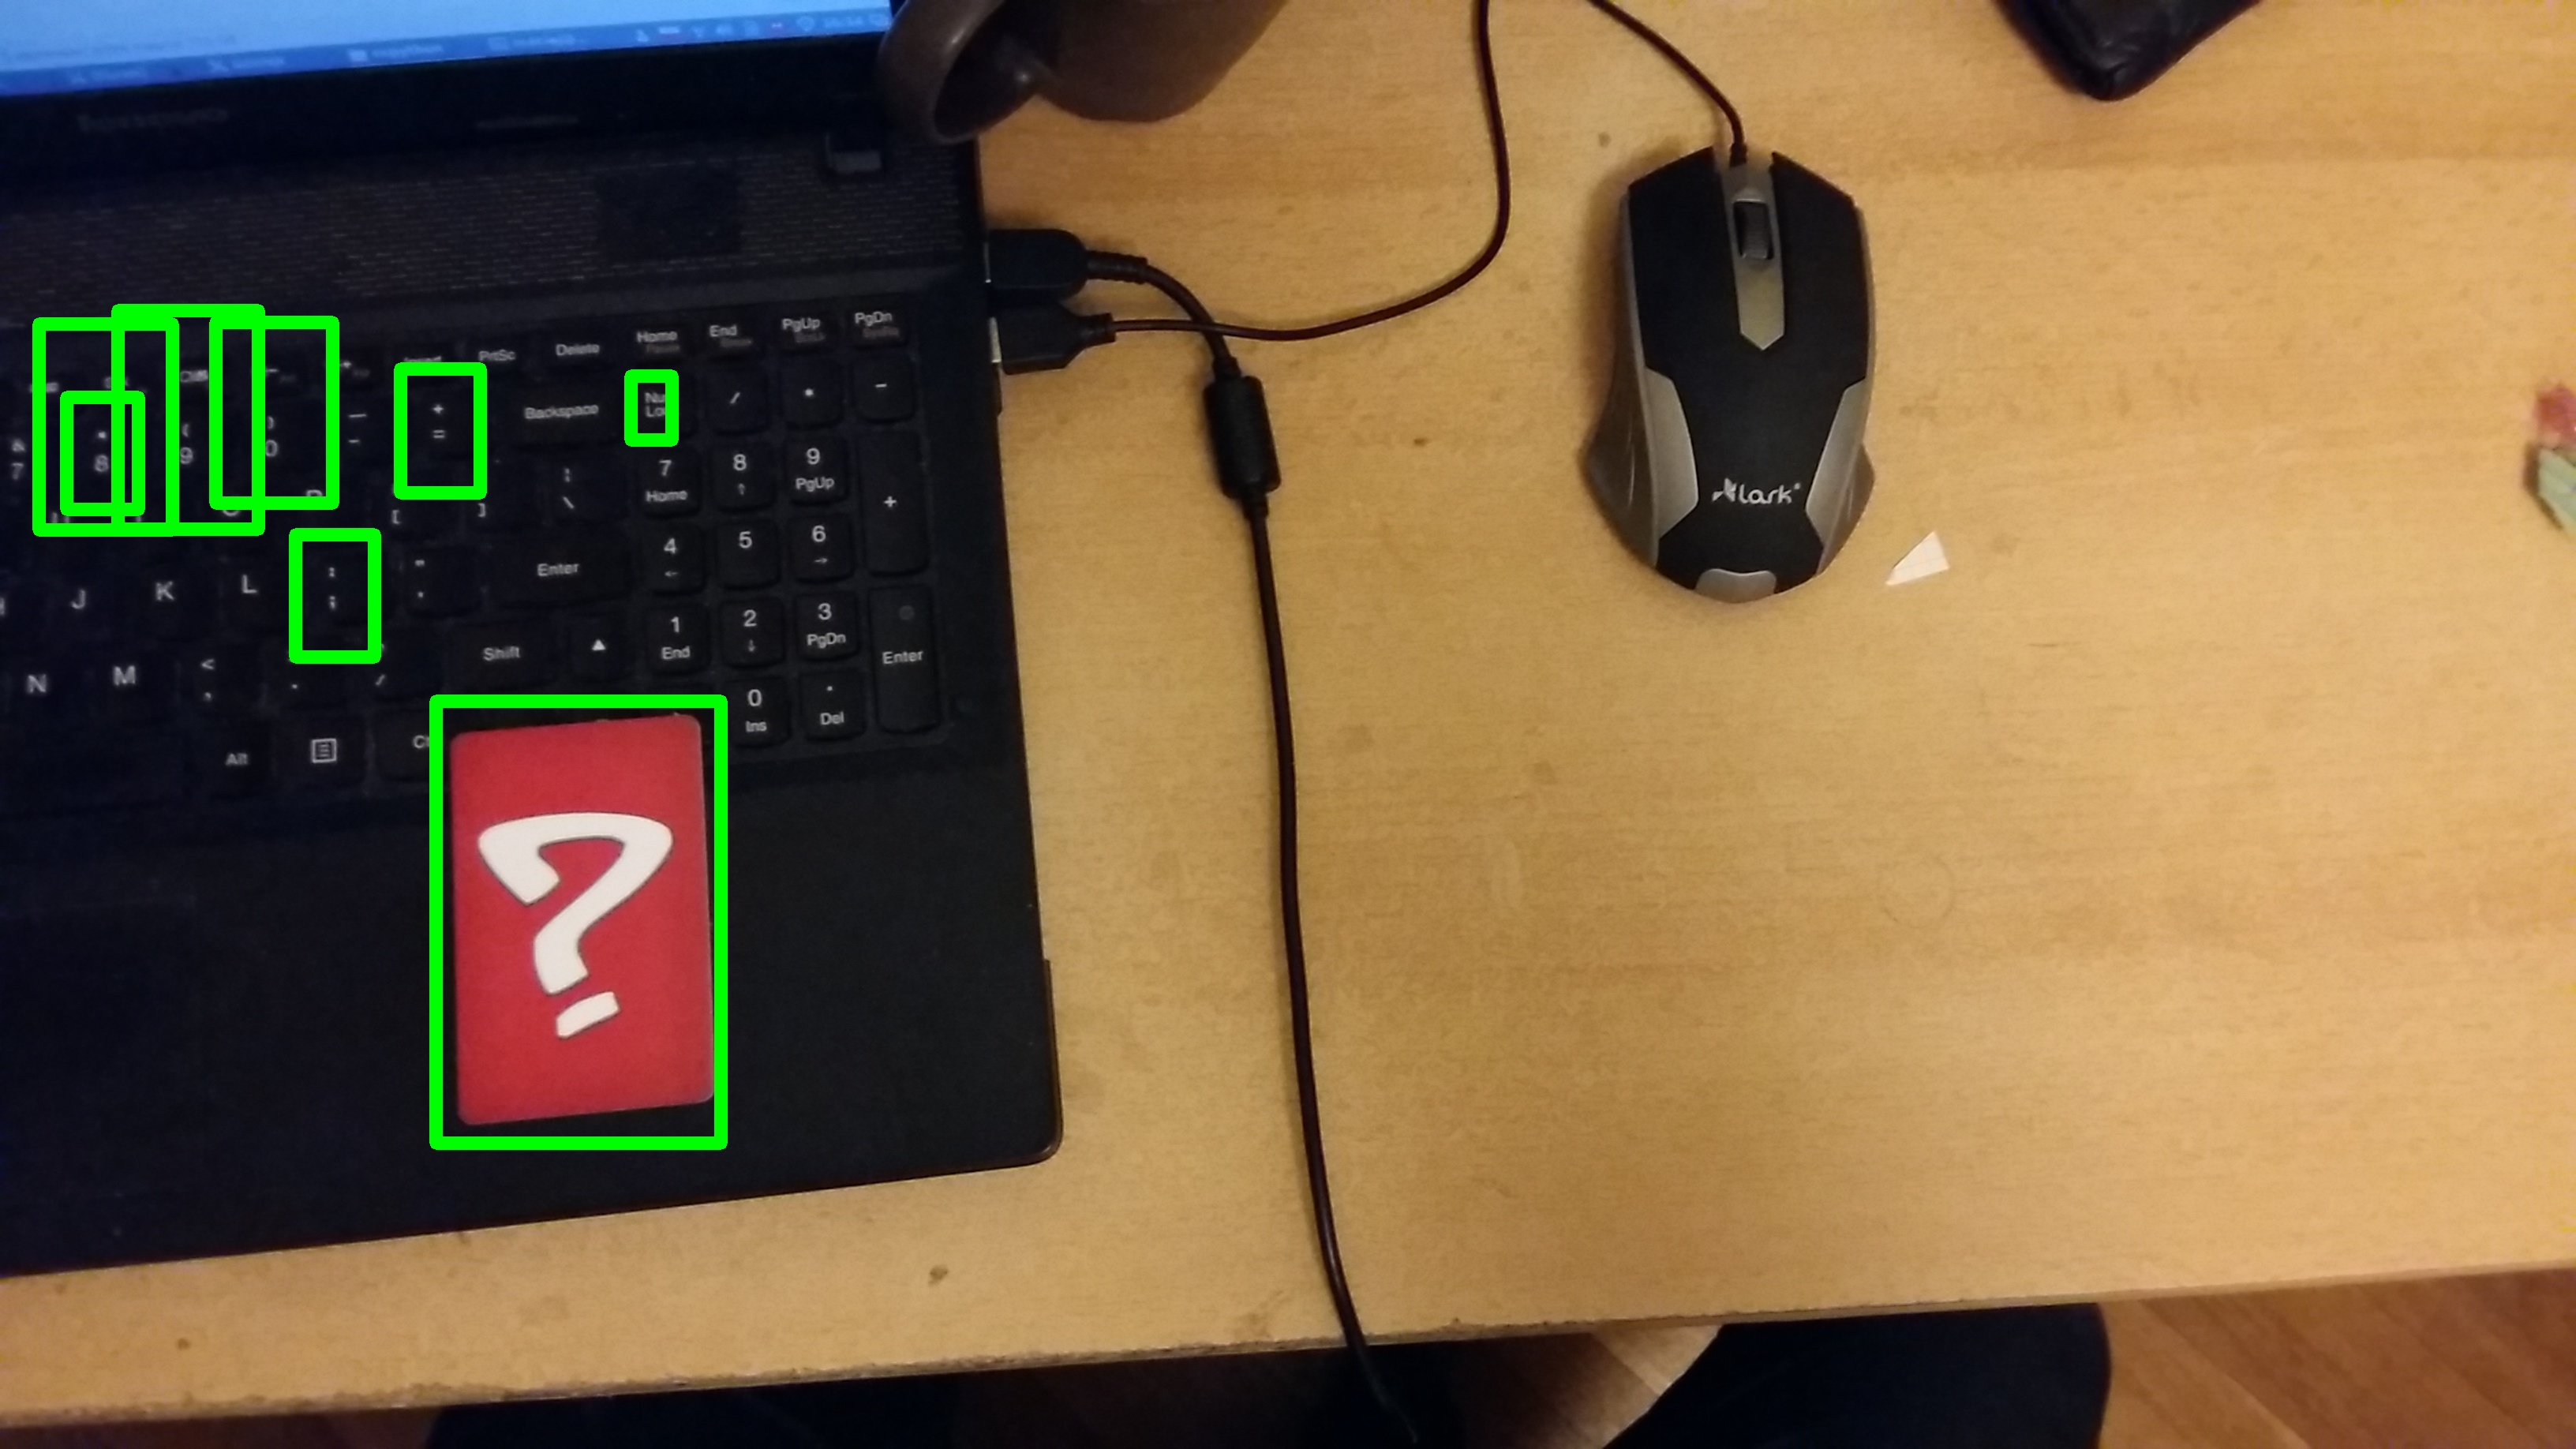
\includegraphics[width=\linewidth]{imgs/karty11.jpg}
        \caption{skala 1.1}
        \label{fig:skalaKarta11}
    \end{subfigure}\hfill
    \begin{subfigure}{0.32\textwidth}
        \centering
        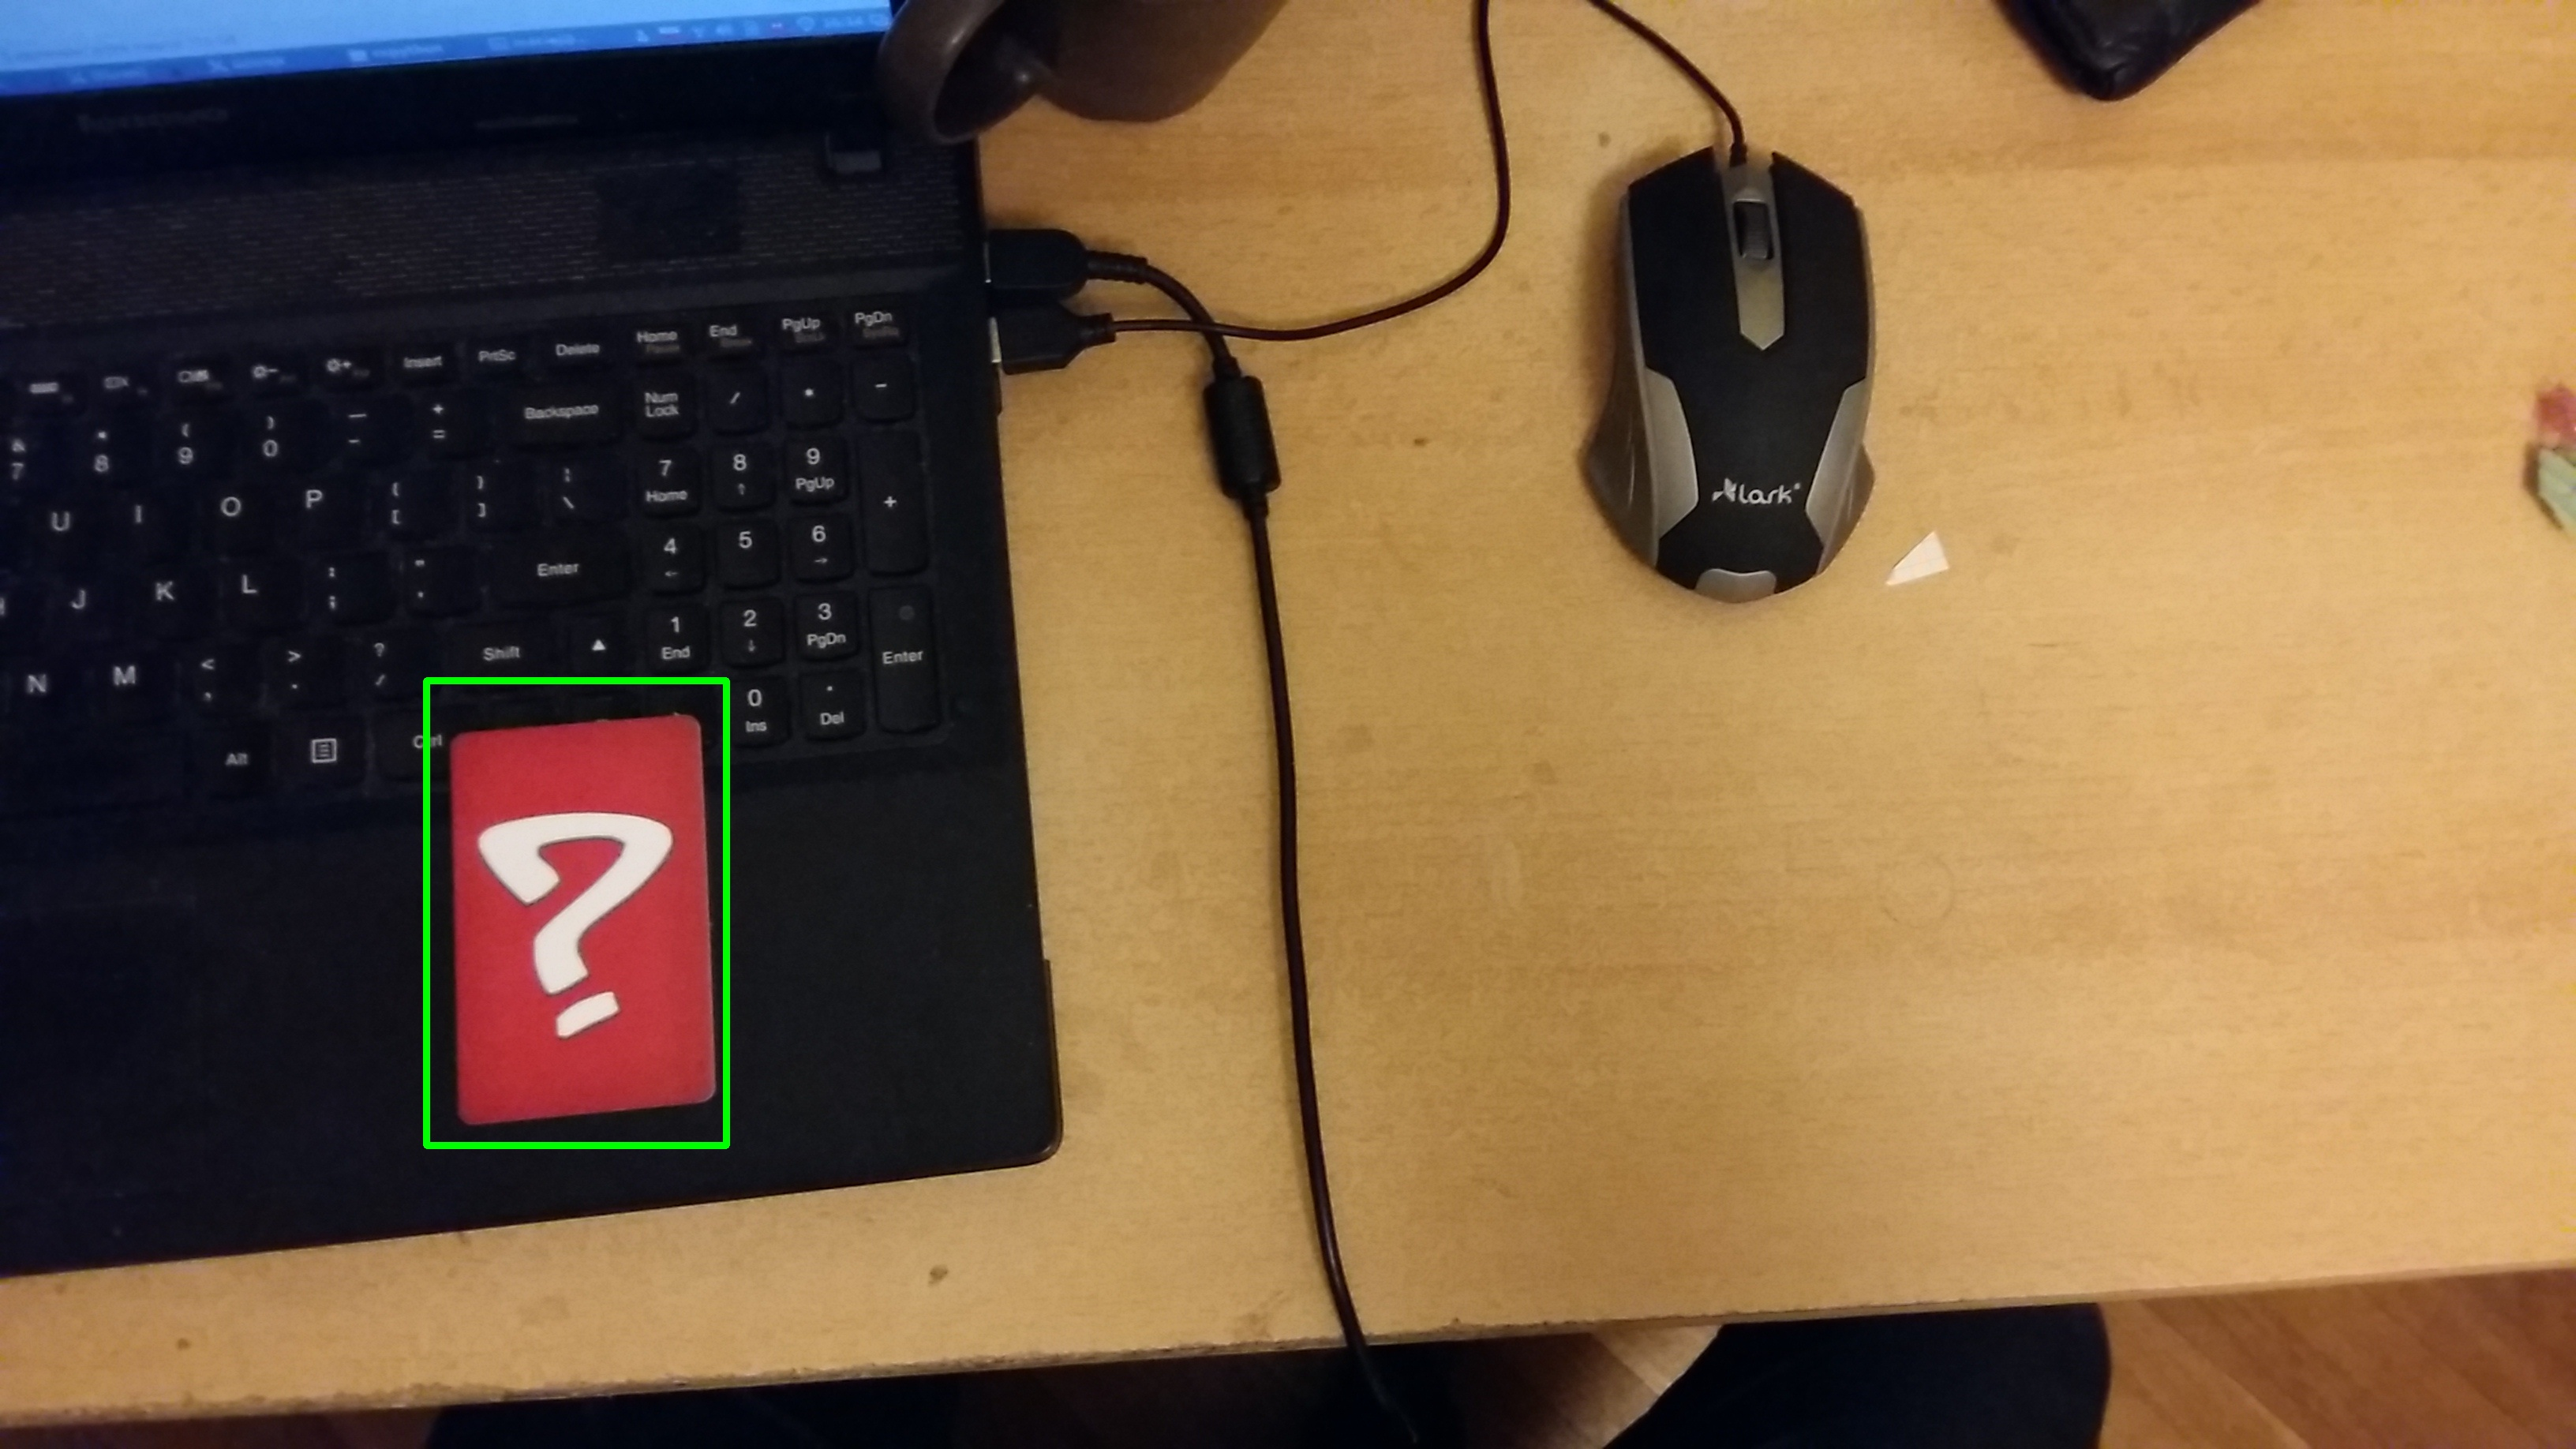
\includegraphics[width=\linewidth]{imgs/karta13.jpg}
        \caption{skala 1.3}
        \label{fig:skalaKarta13}
    \end{subfigure}\hfill
    \begin{subfigure}{0.32\textwidth}
        \centering
        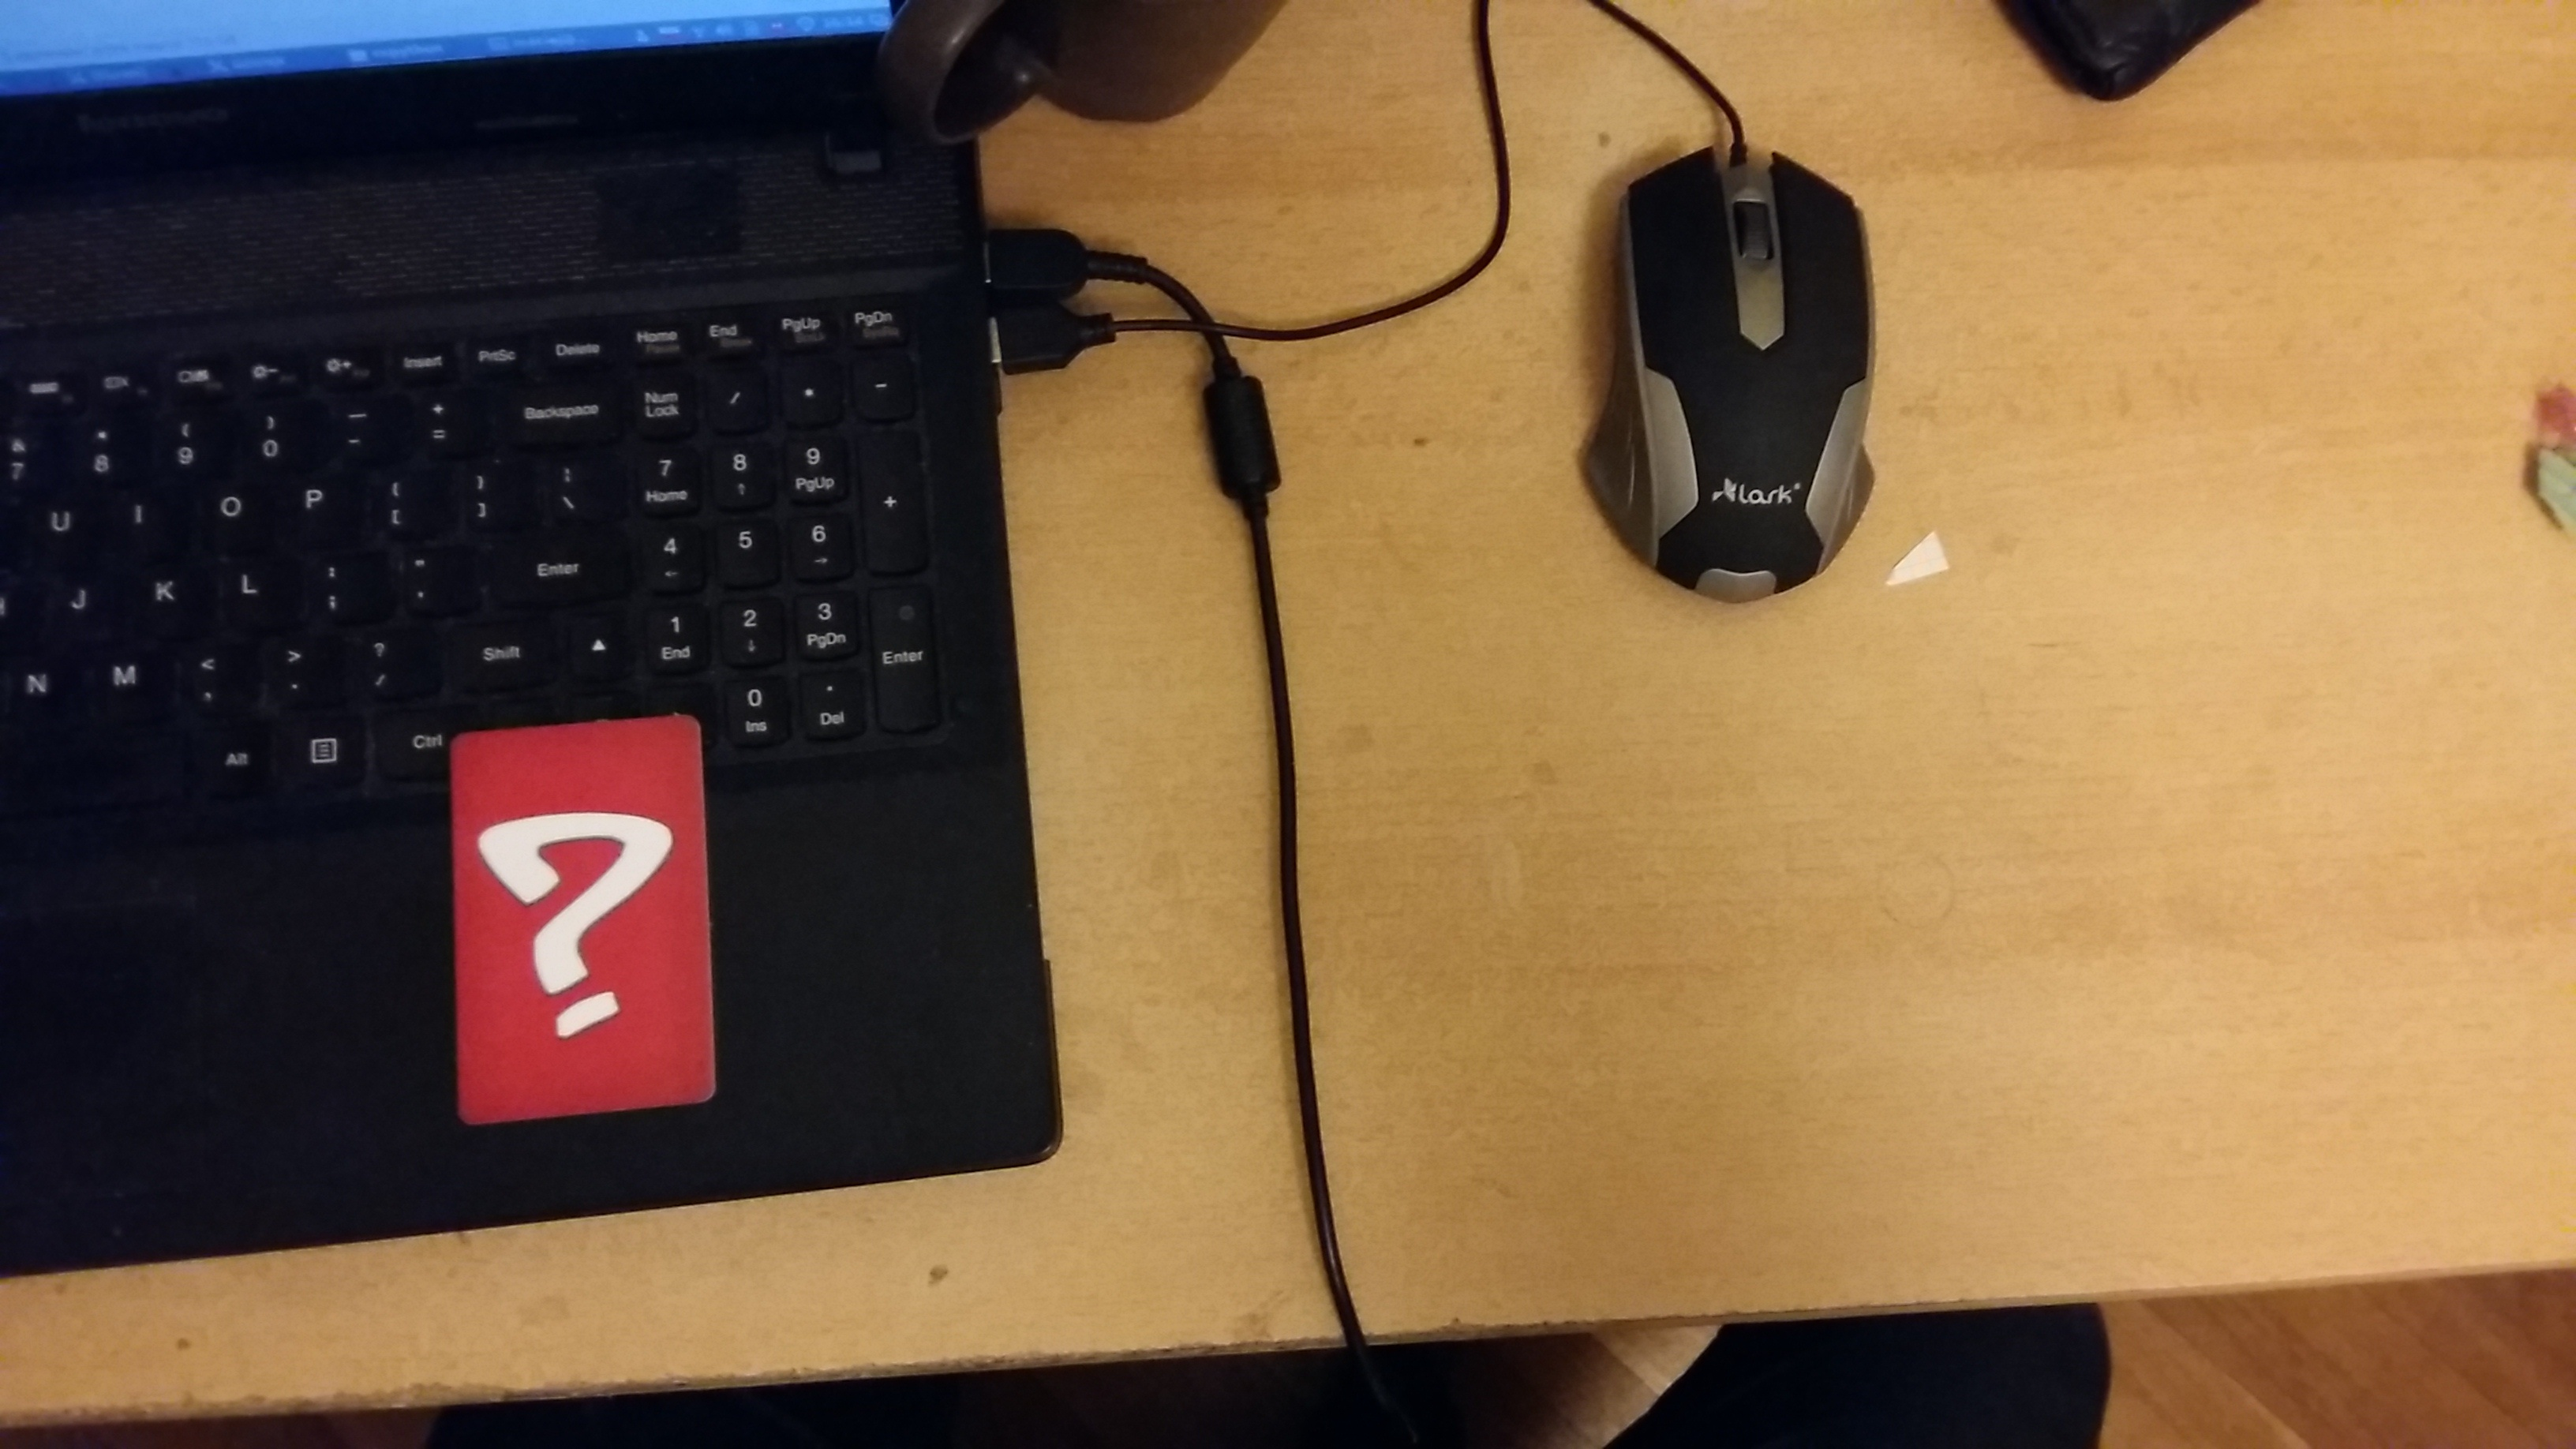
\includegraphics[width=\linewidth]{imgs/kartaaskala20.jpg}
        \caption{skala 2.0}
        \label{fig:skalaKarta20}
    \end{subfigure}
    \caption{Detekcja karty dla różnych wartości scaleFactor}
    \label{kartyy}
\end{figure}

\begin{table}[H]
    \caption{Wyniki detekcji w zalezności od parametru scaleFactor}
    \label{tab:skale}
    \begin{tabular}{|l|c|c|c|c|c|c|c|}
\hline
Rysunek & \ref{fig:twarzSkala11} & \ref{fig:twarzSkala13} & \ref{fig:twarzSkala16} & \ref{fig:skalaKarta11} & \ref{fig:skalaKarta13} & \ref{fig:skalaKarta20}\\
\hline
Skala & 1.1 & 1.3 & 1.6 & 1.1 & 1.3 & 2.0\\
\hline
Czas & 379,397 & 161,874 & 105,139 & 475,516 & 215,779 & 108,829\\
\hline
$F_{pos}$ & 3 & 0 & 0 & 7 & 0 & 0\\
\hline
$F_{neg}$ & 0 & 0 & 3 & 0 & 0 & 1\\
\hline
\end{tabular}
\end{table}

Rysunki \ref{twarzee} i \ref{kartyy} przedstawiają wyniki detekcji twarzy oraz karty dla różnych parametrów scaleFactor. W tabeli \ref{tab:skale} przedstawiono czas detekcji, liczbę błędnych klasyfikacji jako obiekt oznaczonych jako ${F_{pos}}$ oraz liczbę błędnych klasyfikacji jako nie obiekt ${F_{neg}}$ Jak widać im mniejszy parametr tym czas krótszy, ${F_{pos}}$ także się zmniejsza natomiast rośnie wartość ${F_{neg}}$.

Parametr minNeighbors określa w ilu sąsiednich ramkach został odnaleziony obiekt, dopiero przy odpowiedniej liczbie tych sąsiadów podejmowana jest decyzja o znalezieniu wzoru. Zwiększanie tego współczynnika zmniejsza prawdopodobieństwo podjęcia błędnej decyzji o poprawnej detekcji, natomiast zwiększa ryzyko pominięcia elementu.


\begin{figure}[H]
    \centering
        \begin{subfigure}{0.32\textwidth}
        \centering
        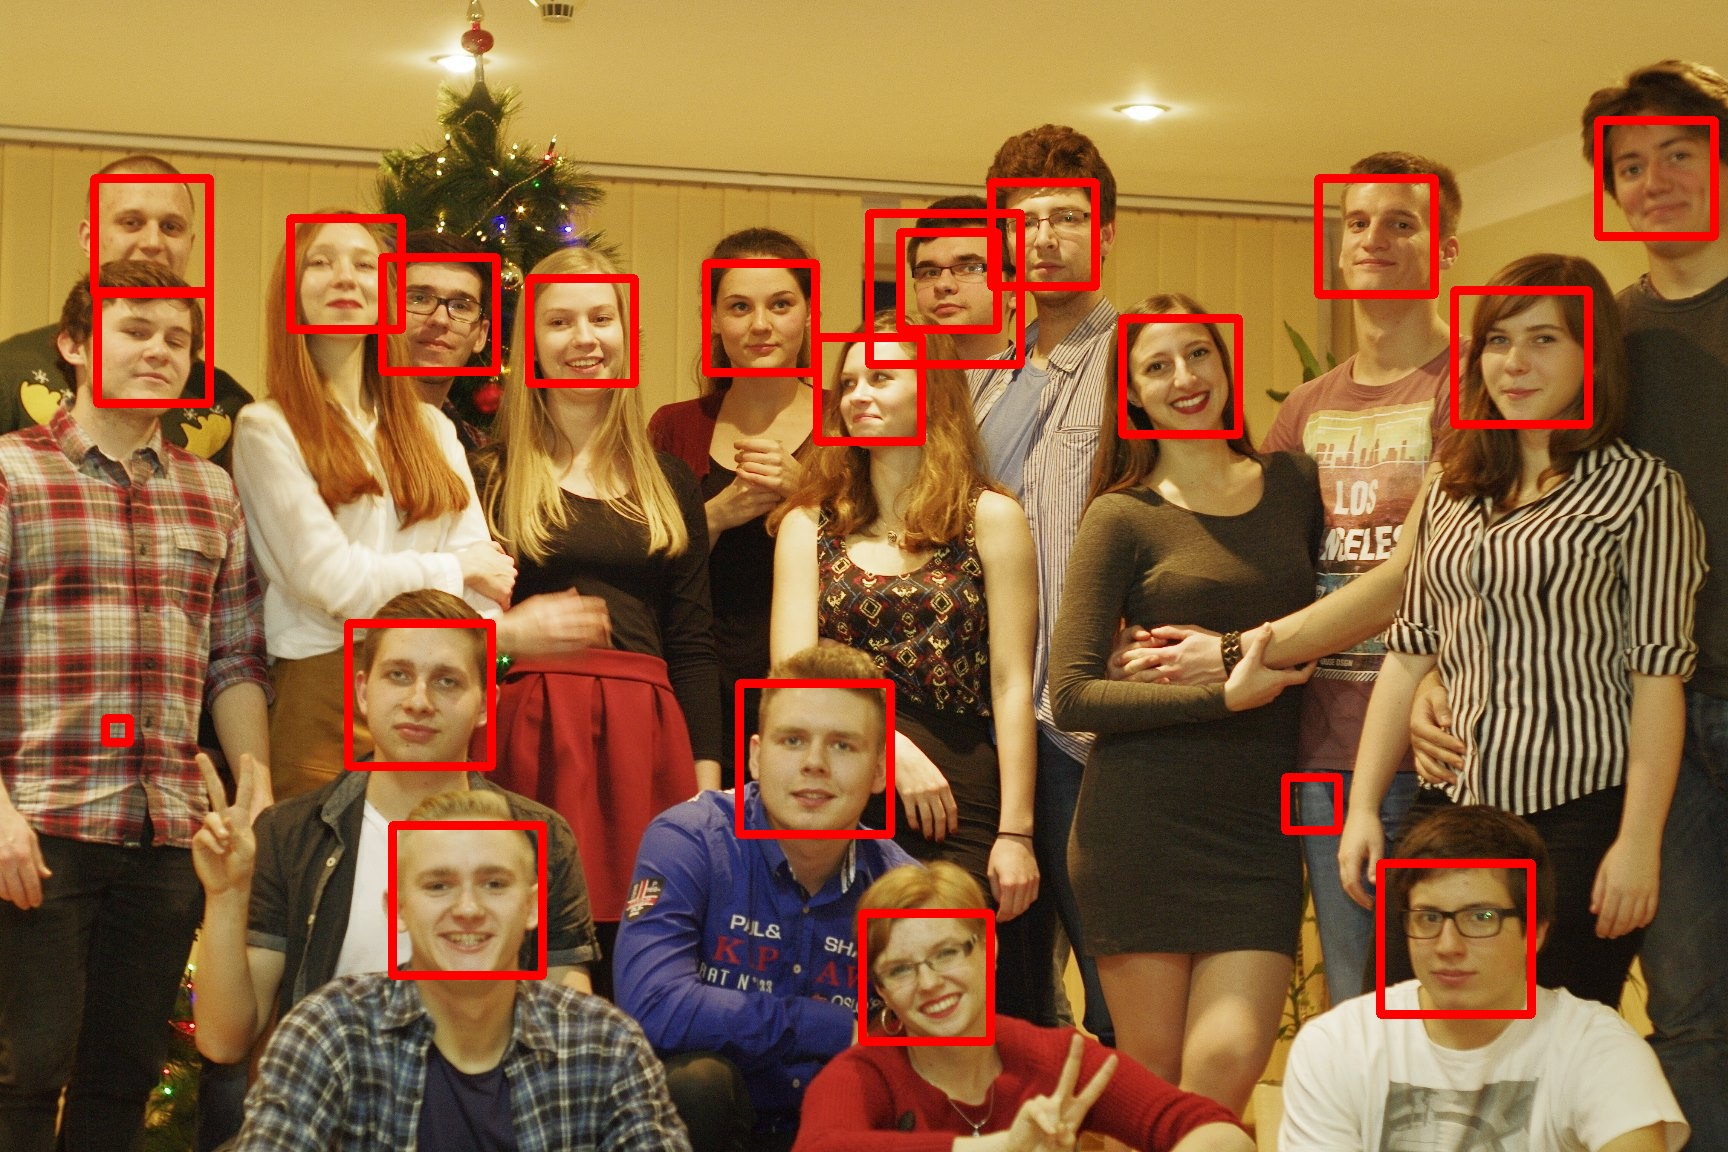
\includegraphics[width=\linewidth]{imgs/somsiad1.jpg}
        \caption{minNeighbors równe 1}
        \label{fig:somsiadTwarze1}
    \end{subfigure}\hfill
    \begin{subfigure}{0.32\textwidth}
        \centering
        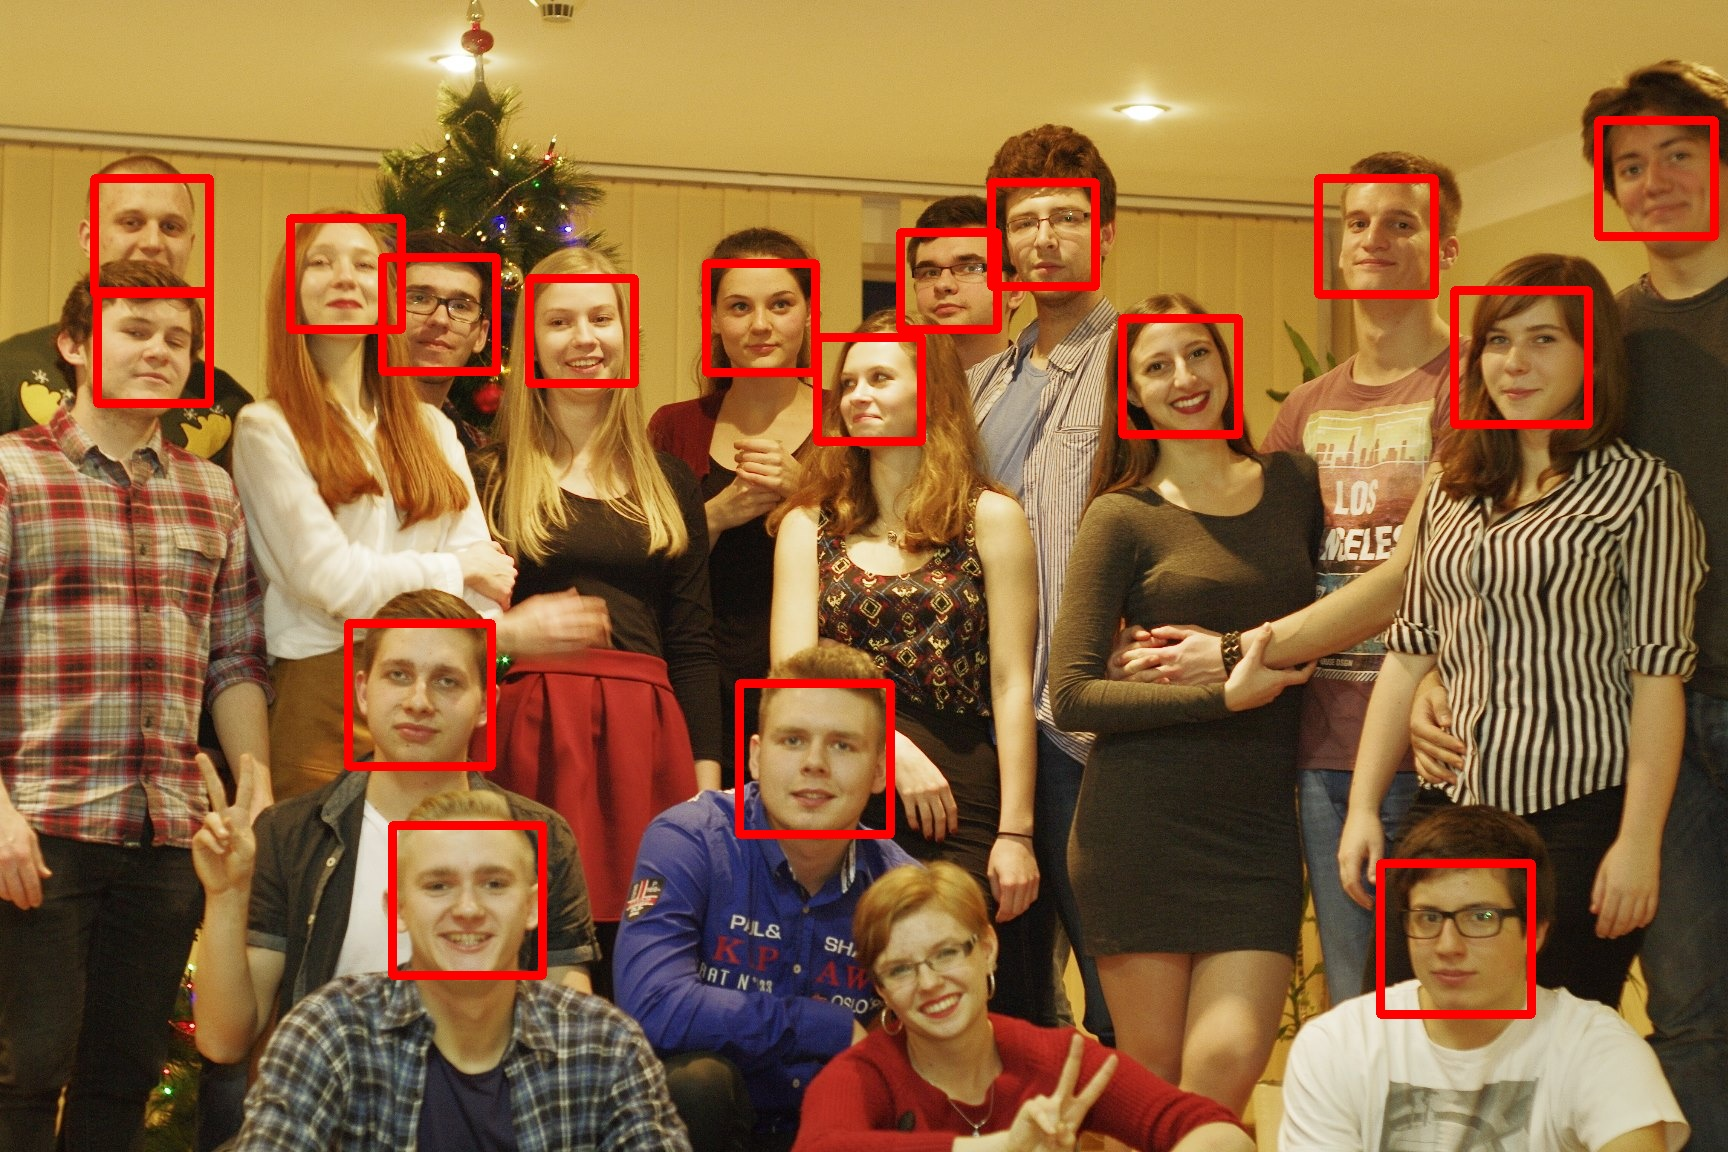
\includegraphics[width=\linewidth]{imgs/somsiad3.jpg}
        \caption{minNeighbors równe 3}
        \label{fig:somsiadTwarze3}
    \end{subfigure}\hfill
    \begin{subfigure}{0.32\textwidth}
        \centering
        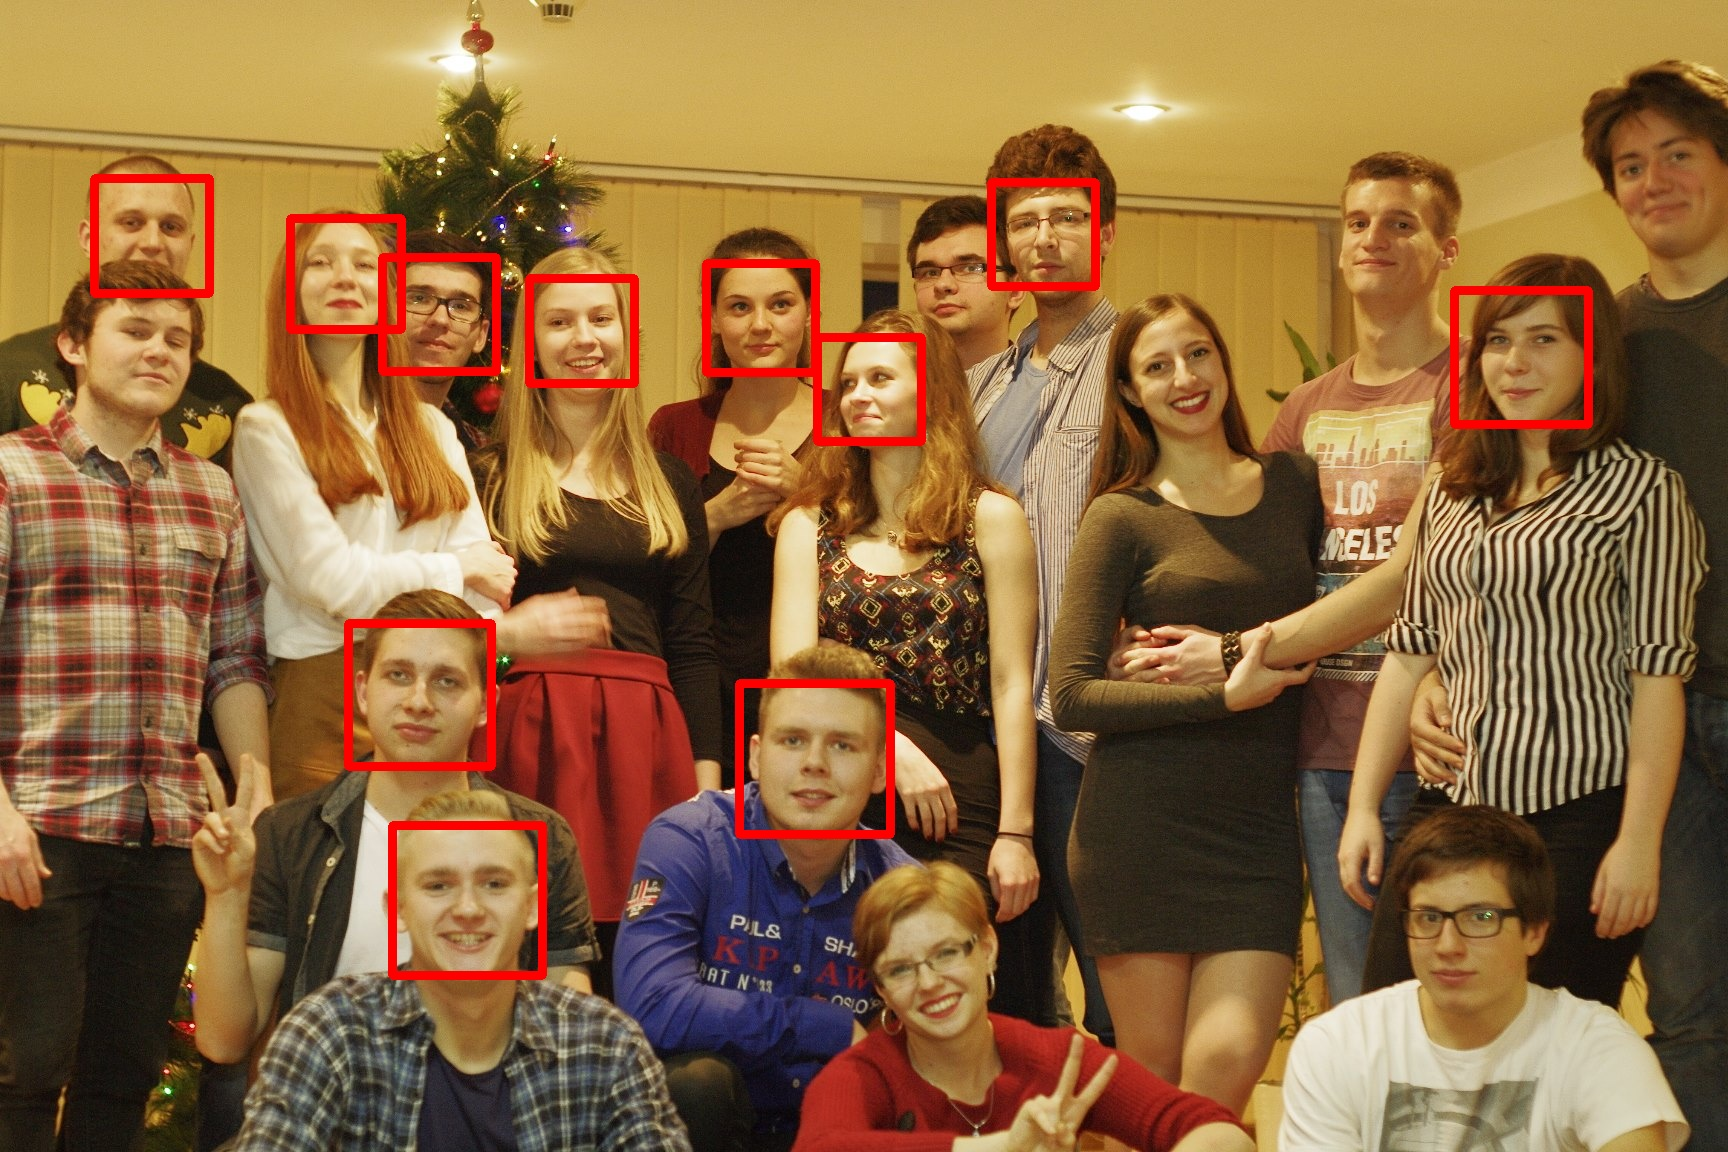
\includegraphics[width=\linewidth]{imgs/somsiad8.jpg}
        \caption{minNeighbors równe 8}
        \label{fig:somsiadTwarze8}
    \end{subfigure}
    \caption{Detekcja twarzy dla różnych wartości minNeighbors}
    \label{twarzeeSomsiady}
\end{figure}

\begin{figure}[H]
    \centering
        \begin{subfigure}{0.32\textwidth}
        \centering
        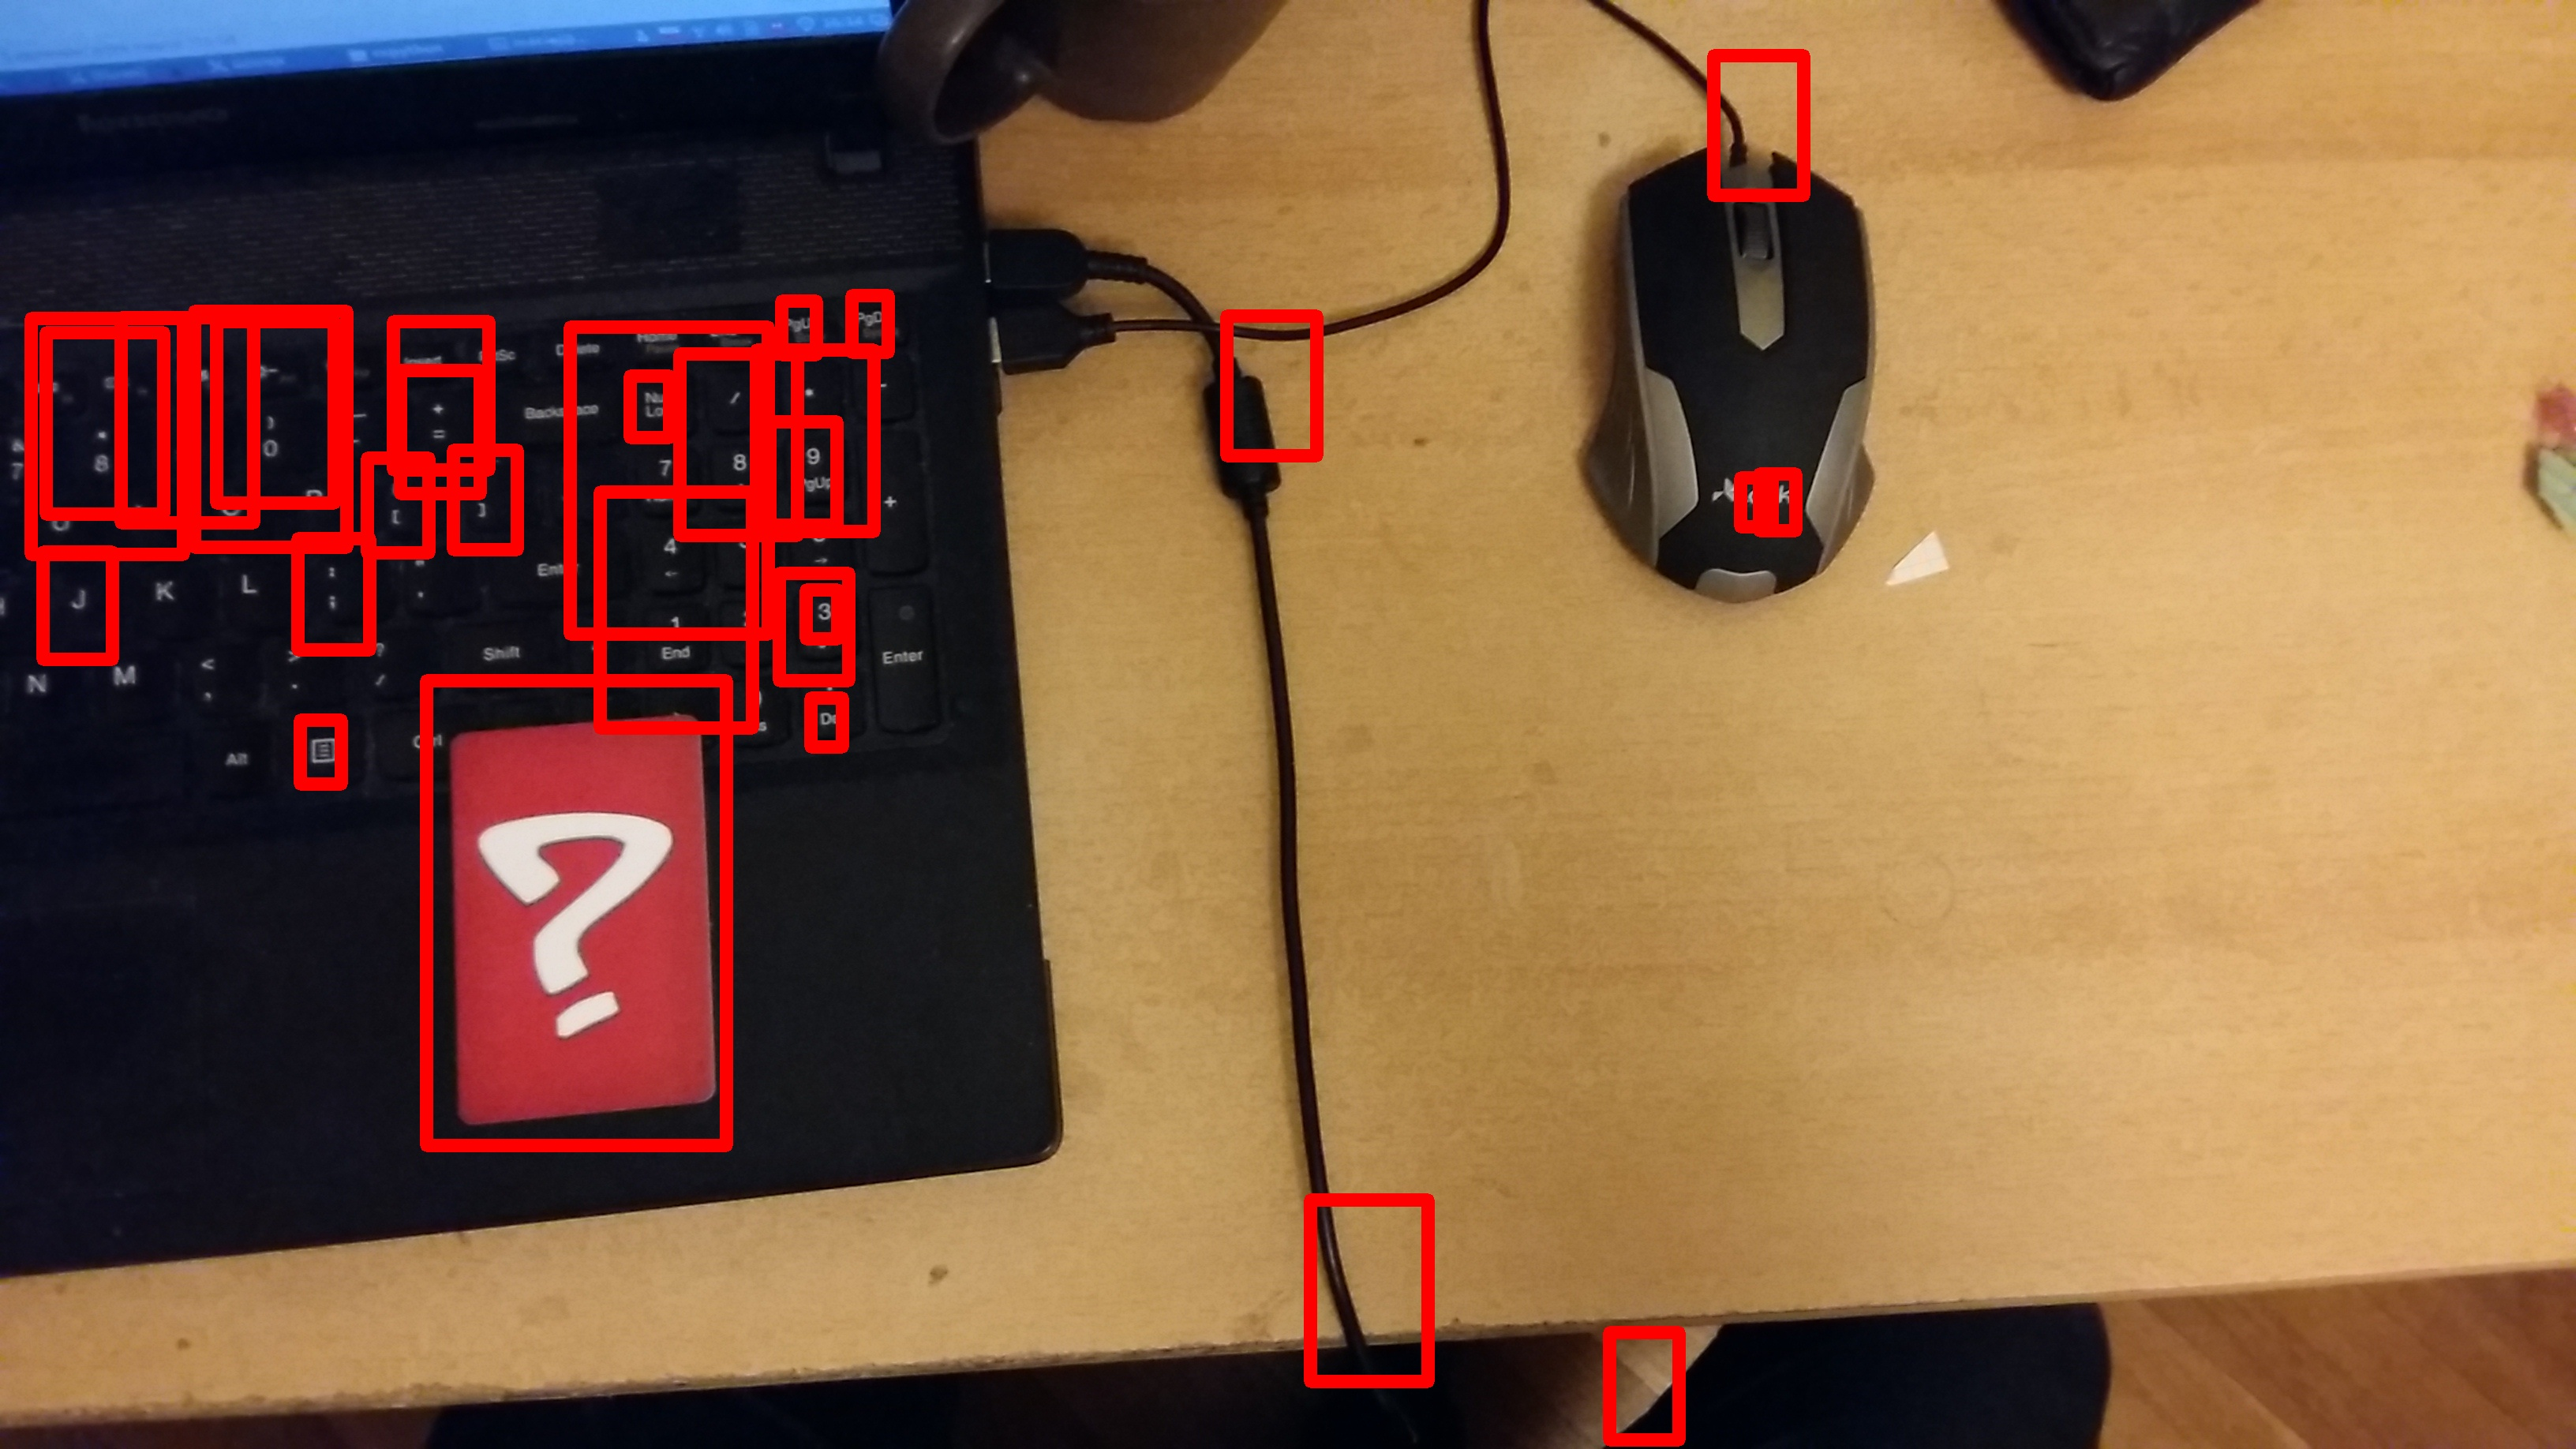
\includegraphics[width=\linewidth]{imgs/somsiadd1.jpg}
        \caption{minNeighbors równe 1}
        \label{fig:somsiadKarta1}
    \end{subfigure}\hfill
    \begin{subfigure}{0.32\textwidth}
        \centering
        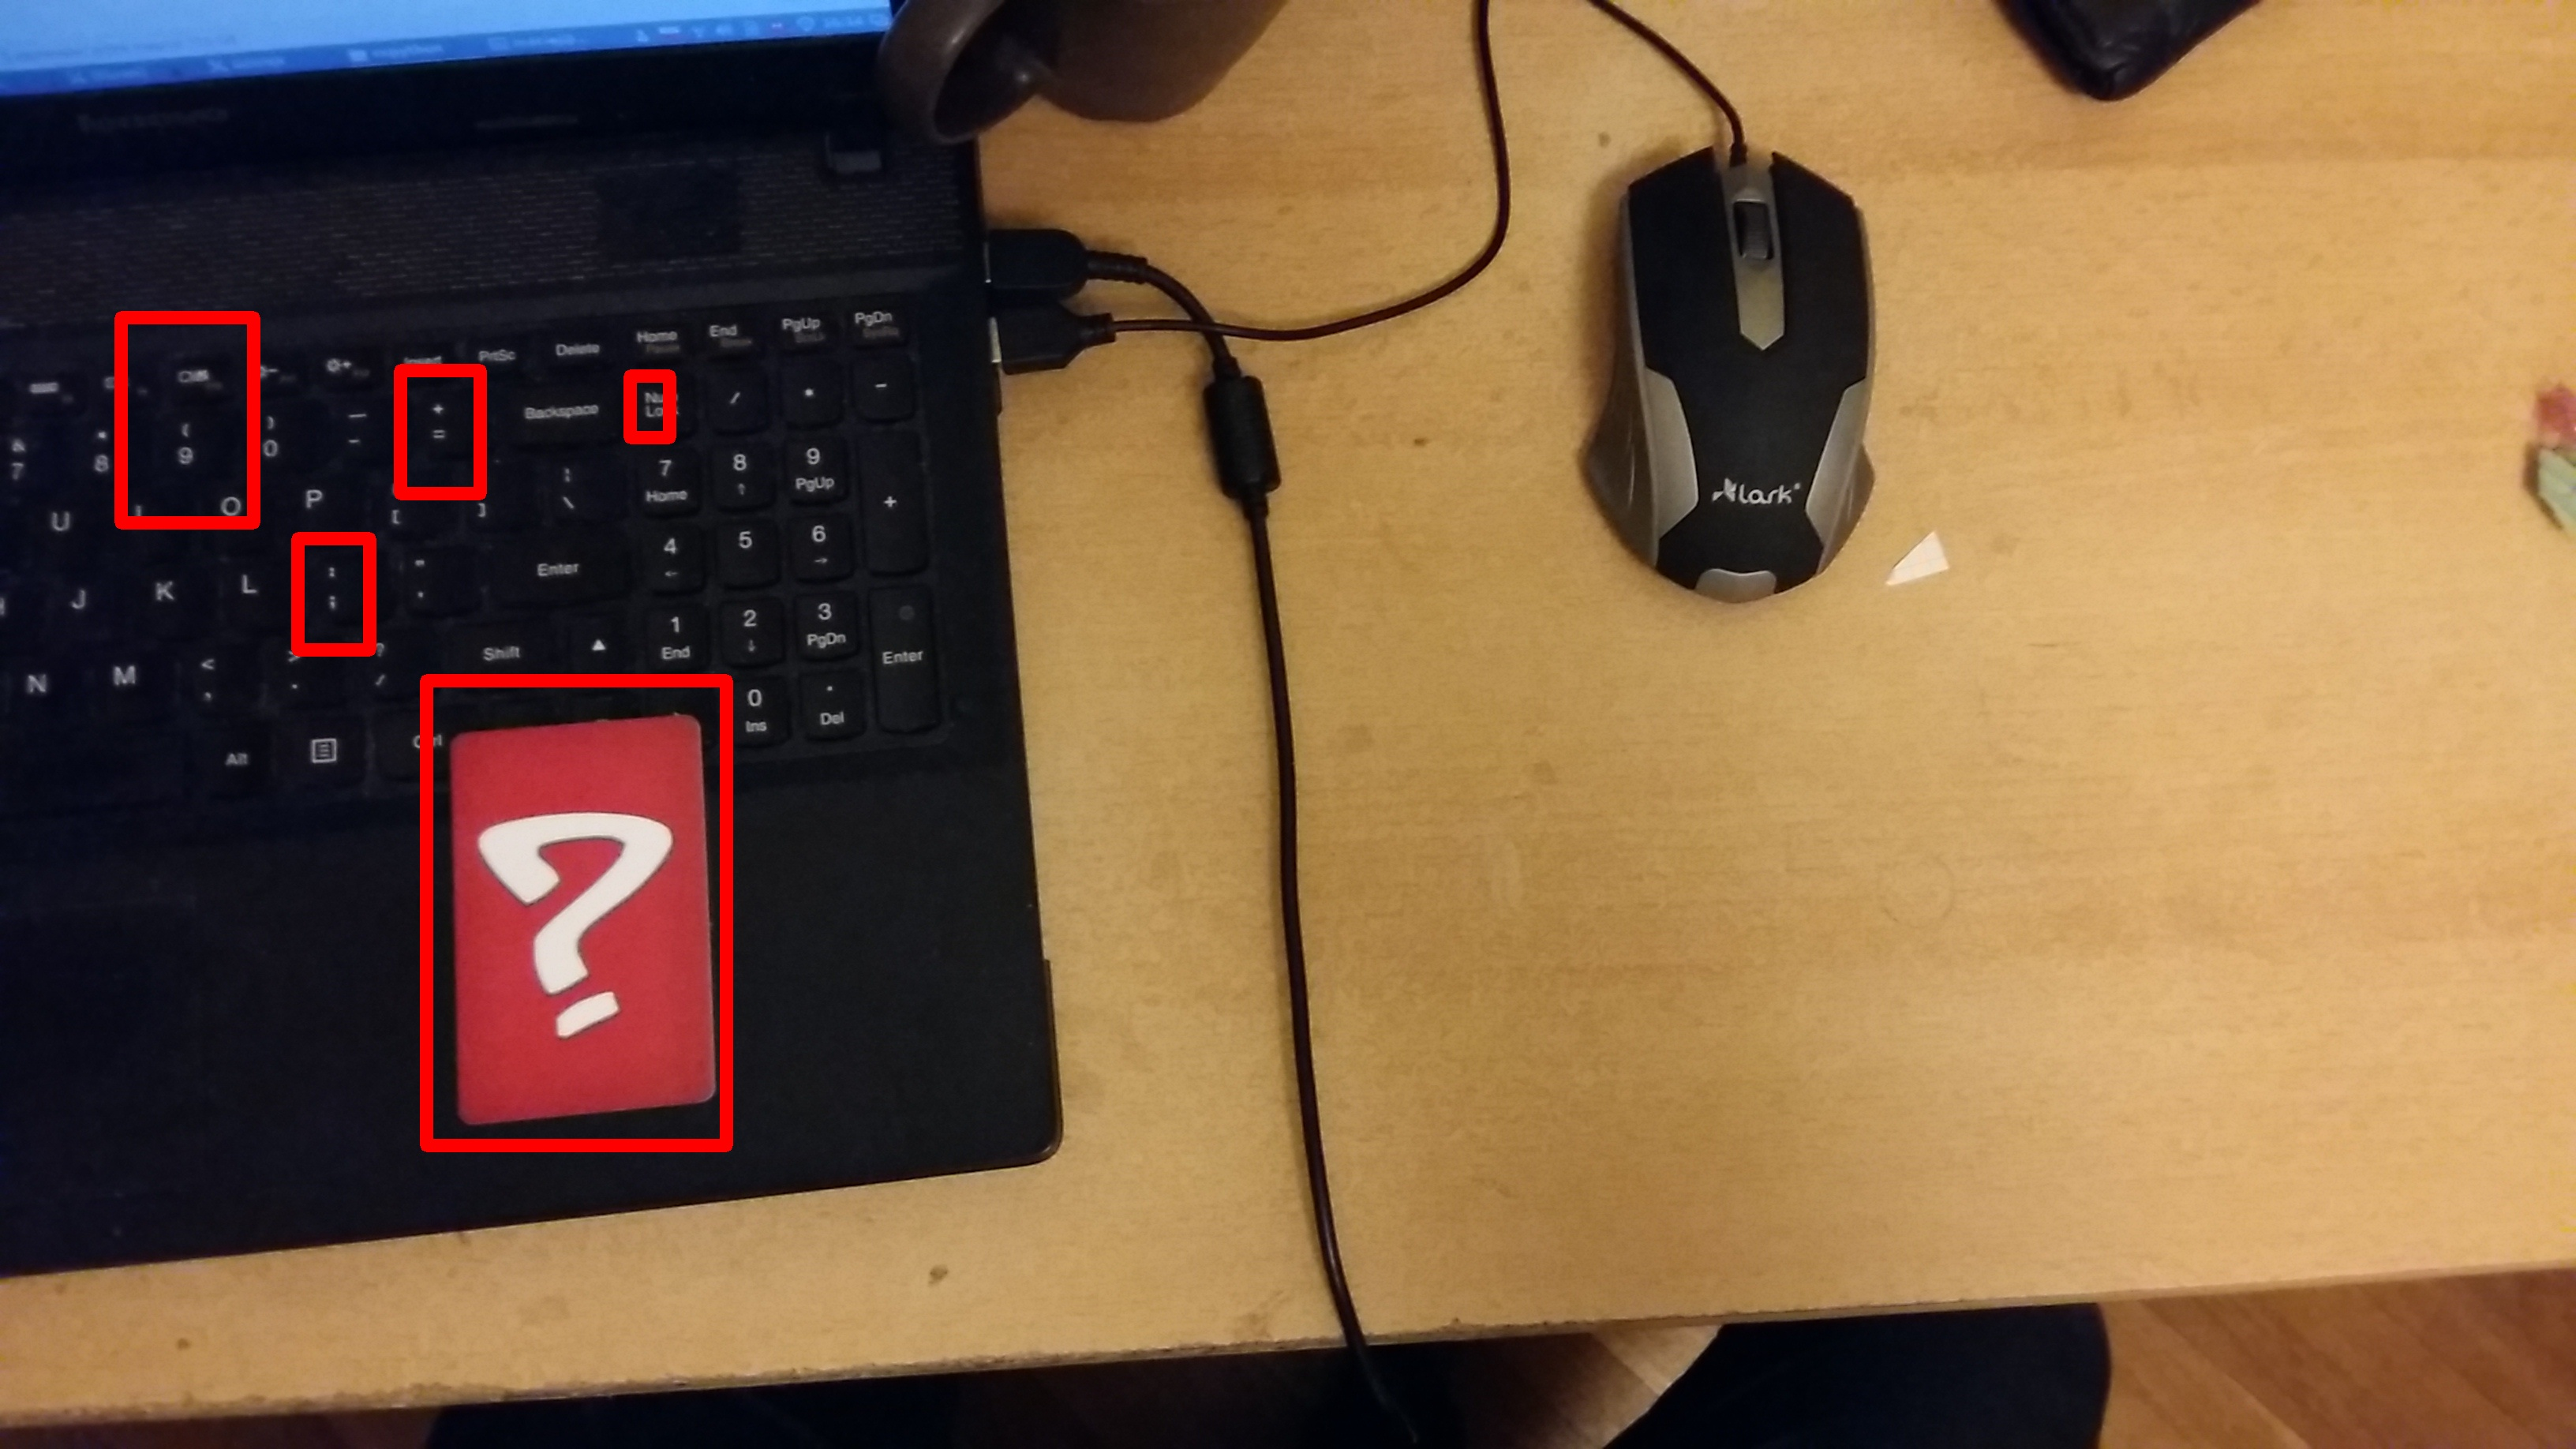
\includegraphics[width=\linewidth]{imgs/somsiadd6.jpg}
        \caption{minNeighbors równe 6}
        \label{fig:somsiadKarta6}
    \end{subfigure}\hfill
    \begin{subfigure}{0.32\textwidth}
        \centering
        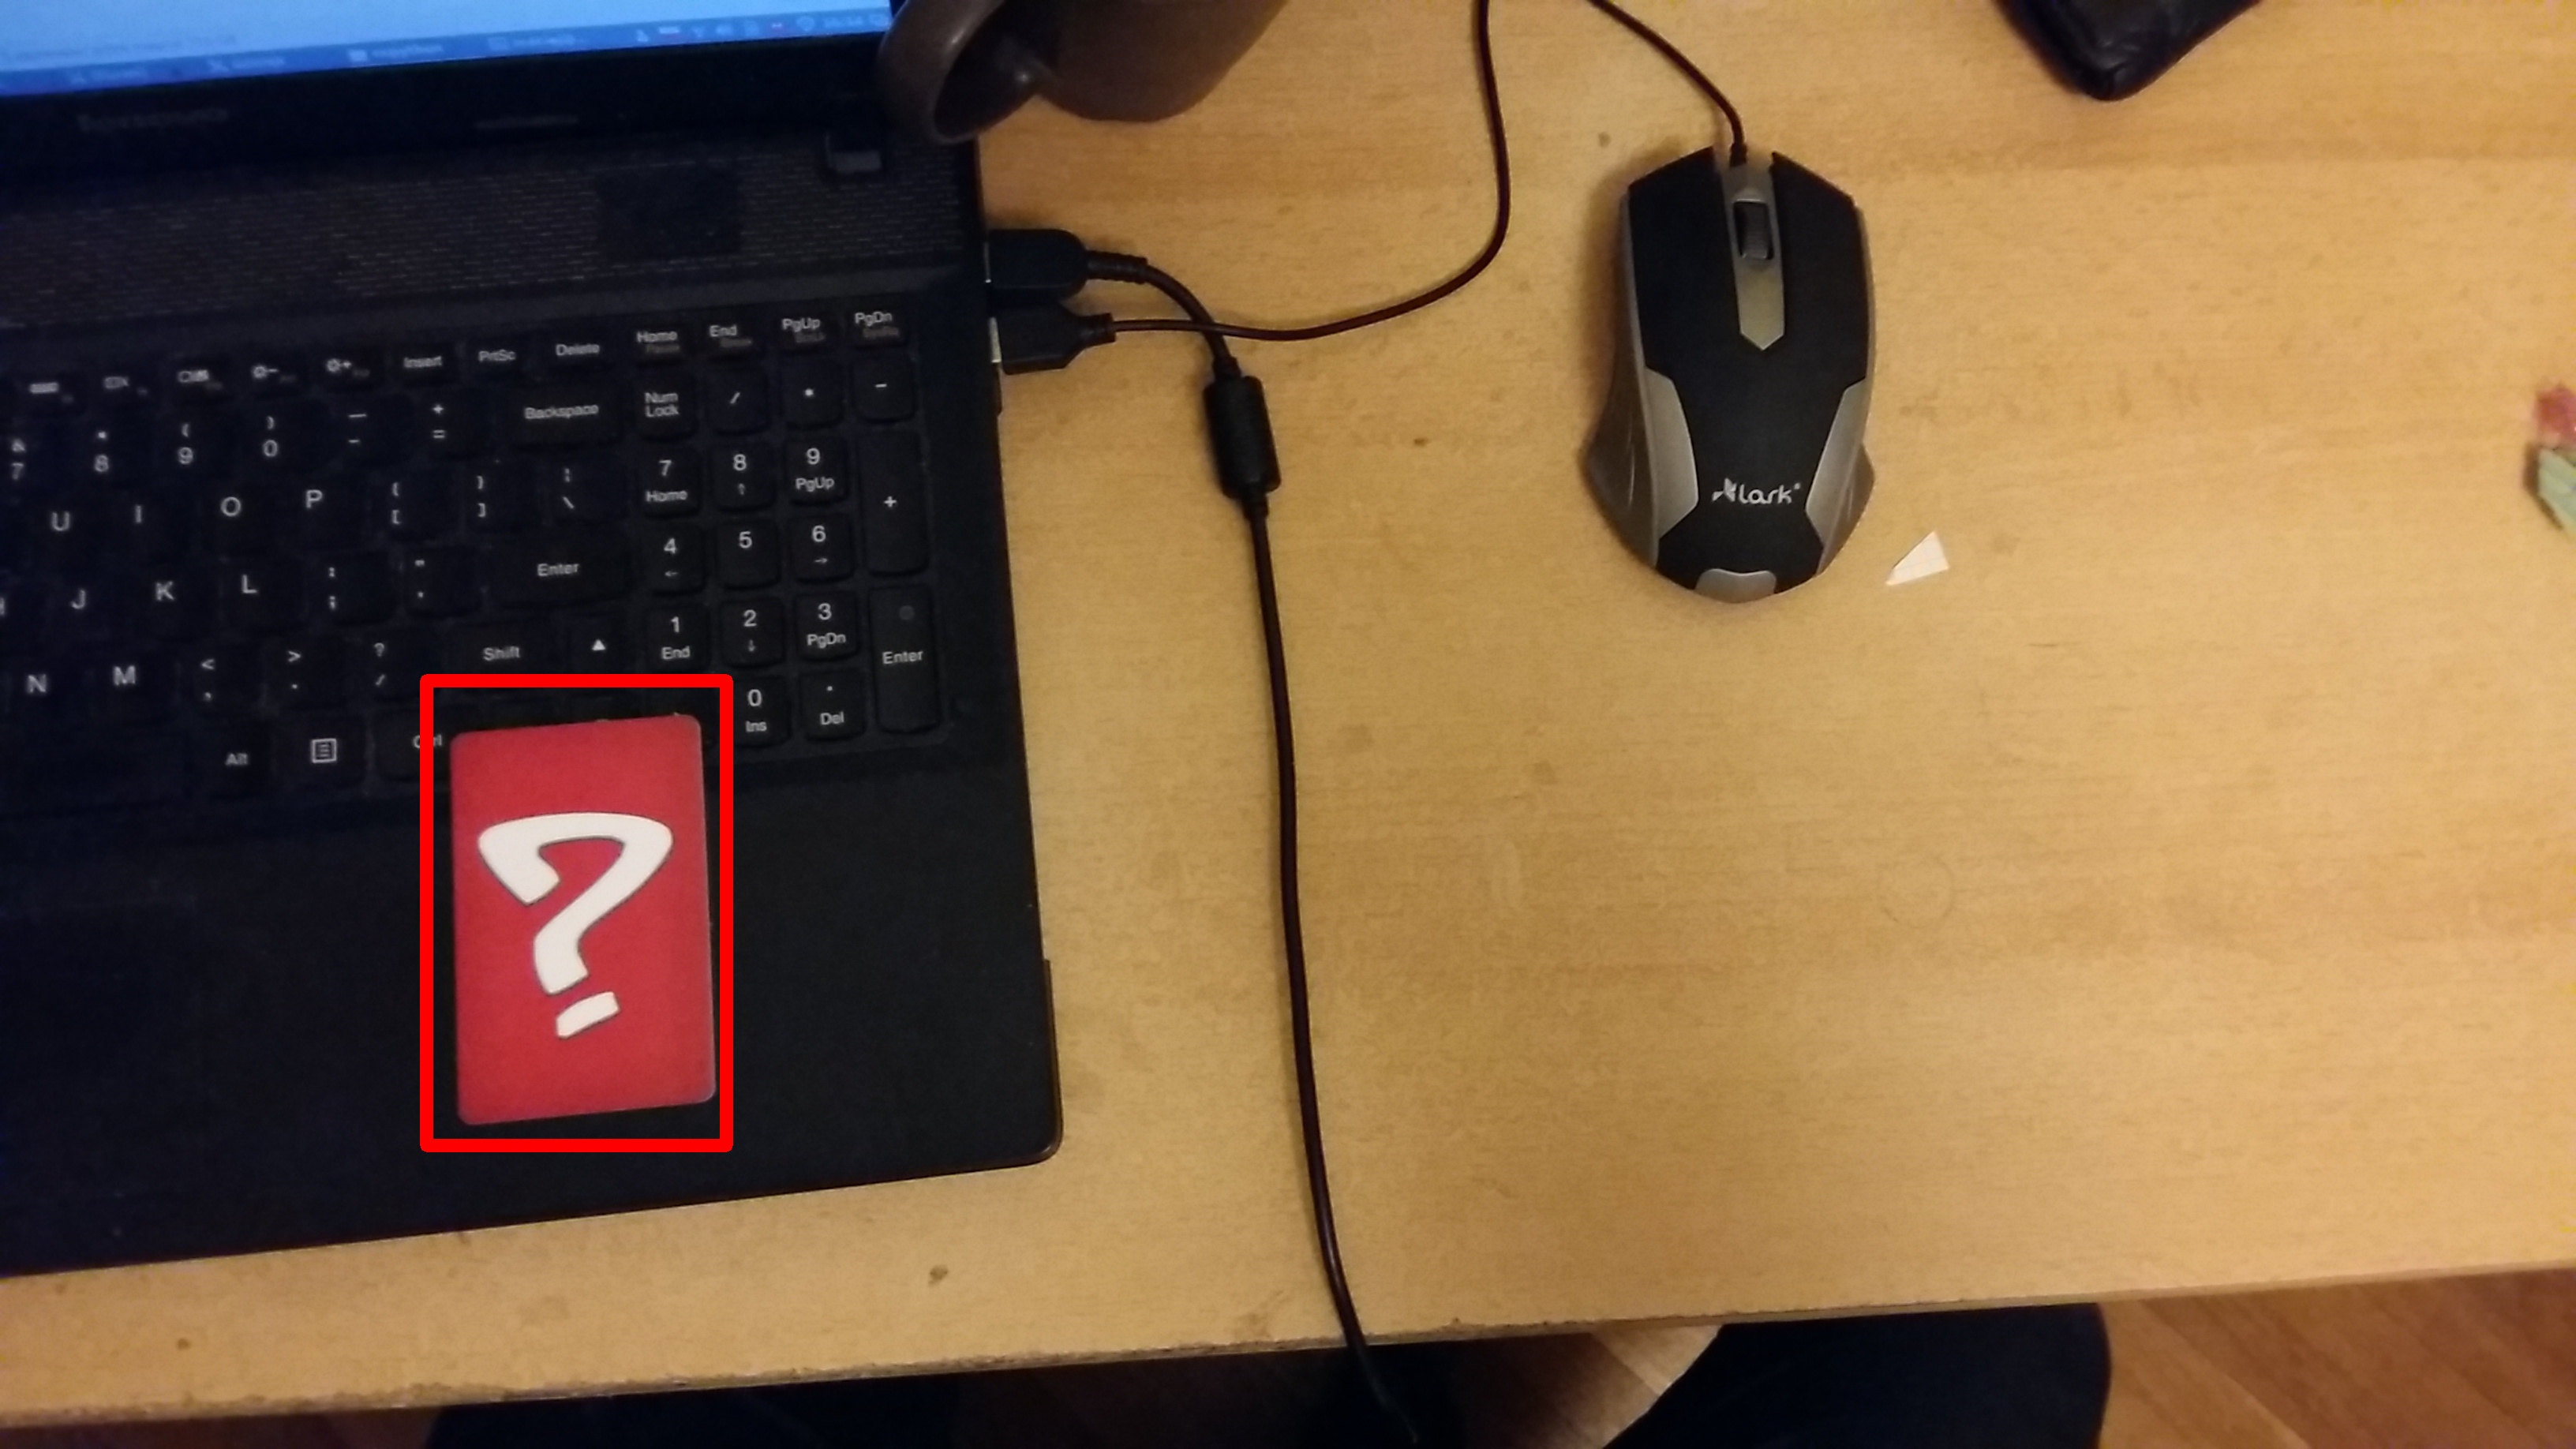
\includegraphics[width=\linewidth]{imgs/somsiadd16.jpg}
        \caption{minNeighbors równe 16}
        \label{fig:somsiadKarta16}
    \end{subfigure}
    \caption{Detekcja karty dla różnych wartości minNeighbors}
    \label{kartySomsiady}
\end{figure}


\begin{table}[H]
    \caption{Wyniki detekcji w zależności od parametru minNeighbors}
    \label{tab:somsiady}
    \begin{tabular}{|l|c|c|c|c|c|c|c|}
\hline
Rysunek & \ref{fig:somsiadTwarze1} & \ref{fig:somsiadTwarze3} & \ref{fig:somsiadTwarze8} & \ref{fig:somsiadKarta1} & \ref{fig:somsiadKarta6} & \ref{fig:somsiadKarta16}\\
\hline
Liczba sąsiadów & 1 & 3 & 8 & 1 & 6 & 16\\
\hline
Czas & 162,046 & 163,162 & 162,370 & 185,266 & 193,285 & 193,086\\
\hline
$F_{pos}$ & 2 & 0 & 0 & 28 & 4 & 0\\
\hline
$F_{neg}$ & 0 & 1 & 6 & 0 & 0 & 0\\
\hline
\end{tabular}
\end{table}

Rysunki \ref{twarzeeSomsiady} - \ref{kartySomsiady} przedstawiają wyniki detekcji twarzy oraz karty dla różnych parametrów minNeighbors. W tabeli \ref{tab:somsiady} przedstawiono rezultaty detekcji dla tych rysunków. Wynika z tego, że zmiana minimalnej liczby sąsiadów nie wpływa na czas detekcji. Przy zmianie parametru można jednak zauważyć dużą zmianę skuteczności. Dla wykrywania twarzy widać mniejszą liczbę ${F_{pos}}$ , stąd też dla mniejszej liczby minimalnych sąsiadów osiągnięto idealny rezultat.
W przypadku detekcji twarzy oraz oczu zdecydowano by zastosowano sugerowane wartości dla tych kaskad, są to:
\begin{itemize}
    \item minNeighbors = 3
    \item -scaleFactor = 1.3
\end{itemize}

Dla detekcji karty postanowiono przetestować dla jakich parametrów osiągnięto najlepszą skuteczność. W tym celu zebrano 10 zdjęć testowych na których znajduje się jedna karta. Na początku postanowiono ustawić parametr minNeighbors.
Zdjęcia przeszły proces detekcji, gdzie parametr minNeighbors przyjmował co drugą wartośc z zakresu <1,40> oraz scaleFactor równemu 1.3. Sprawdzano jaką liczbę odnalezionych obiektów. W przypadku wskazania jednego obiektu nie będącym szukaną kartą nie brano takiego pomiaru pod uwagę.

\begin{table}[H]
    \caption{Poszukiwanie najlepszej wartości minNeighbors cz. 1}
    \label{tab:somsiadyNaj1}
    \begin{tabular}{|c|c|c|c|c|c|c|c|c|c|c|}
\hline
minNeighbors & 1 & 3 & 5 & 7 & 9 & 11 & 13 & 15 & 17 & 19\\
\hline
Liczba odnalezionych & 11,62 & 6,89 & 4,89 & 3,68 & 3,03 & 2,86 & 2,51 & 1,89 & 1,68 & 1,82 \\
\hline
\end{tabular}
\end{table}

\begin{table}[H]
    \caption{Poszukiwanie najlepszej wartości minNeighbors cz. 2}
    \label{tab:somsiadyNaj2}
    \begin{tabular}{|c|c|c|c|c|c|c|c|c|c|c|}
\hline
minNeighbors & 21 & 23 & 25 & 27 & 29 & 31 & 33 & 35 & 37 & 39\\
\hline
Liczba odnalezionych &  1,34 & 1,20 & 1,06 & 0,91 & 0,75 & 0,65 & 0,48 & 0,44 & 0,41 & 0,34\\
\hline
\end{tabular}
\end{table}

W tabelach \ref{tab:somsiadyNaj1} i \ref{tab:somsiadyNaj2} przedstawiono średnie wartości liczby odnalezionych obiektów w zależności od parametru minNeighbors. Wynika z nich, że najlepsze decyzje były podejmowane dla wartości 25.
Na podstawie tego wyniku szukano najlepszej wartości parametru scaleFactor. Podobnie jak w poprzednim przypadku użyto tych samych dziesięciu zdjęć. Testowano wartości współczynnika scaleFactor od 1,1 do 1,7 co 0,05.

\begin{table}[H]
    \caption{Poszukiwanie najlepszej wartości scaleFactor}
    \label{tab:ckalaNaj}
    \begin{tabular}{|c|c|c|c|c|c|c|c|c|c|c|c|c|c|}
\hline
minNeighbors & 1.1 & 1.15 & 1.2 & 1.25 & 1.3 & 1.35 & 1.4 & 1.45 & 1.5 & 1.55 & 1.6 & 1.65 & 1.7\\
\hline
Liczba odnalezionych & 3,9 & 2,6 & 2,1 & 1,4 & 1,5 & 1,3 & 1,2 & 1,2 & 1,3 & 0,8 & 0,8 & 0,9& 0,8\\
\hline
\end{tabular}
\end{table}

W tabeli \ref{tab:ckalaNaj} przedstawiono średni wynik ilości odnalezionych obiektów w zależności od parametru scaleFactor. Dla detekcji karty w naszej aplikacji parametr ten będzie wynosił 1.4, ponieważ dla takiego parametru uzyskano najlepszą wartość będącą większą od 1, jednocześnie z pośród innych parametrów dla których uzyskano podobny wynik, ten gwarantuje mniejszą szansę przeoczenia obiektu.

\subsection{Zmniejszanie zdjęcia}
W przypadku naszej aplikacji wymaganie związane ze skutecznością ma większy priorytet niż czas działania. Dlatego pomyślano, że w przypadku kiedy nie zostanie podjęta jednoznaczna decyzja o odnalezieniu dokładnie jednego przedmiotu należy pomniejszyć zdjęcie i ponownie spróbować odnaleźć obiekt. Działanie takie podjęto ponieważ kaskada została wytrenowana na podstawie pomniejszonych zdjęć, więc powinna lepiej generalizować dla zdjęć pomniejszonych. W celu sprawdzenia tej teorii zebrano 10 zdjęć, dla których nie udało się wskazać dokładnie jednego obiektu, tak jak powinno zostać określone. Algorytm zakłada, że jeśli nie odnaleziono dokładnie jednego elementu, wysokosc i szerokosc zdjęcia dzielona jest przez 1,5. Następnie ponownie przeprowadzana jest detekcja obiektu. Proces ten się zakończy jeśli na którymś z etapów odnaleziono obiekt, lub szerokość osiągnie wartość minimalną, ustaloną na 120 pikseli. W rezultacie testu okazało się, że dla sześciu z dziesięciu zdjęć, w których przy oryginalnym rozmiarze wynik detekcji był niepoprawny, dla pomniejszonego zdjęcia udało się poprawnie odnaleźć obiekt. Operacja zmiany wielkości zdjęcia jest kosztowna jednak trwa znacznie krócej niż wykonanie ponownego zdjęcia i przeprowadzenie dla niego detekcji. Algorytm służący do testowania przeniesiono do kodu aplikacji co znacząco poprawiło skuteczność

\subsection{Wklejanie obrazu karty w miejsce obiektu}

Obrazy całej talii kart znajdują się zasobach aplikacji. Każdy z obrazów ma przypisane unikalne ID. Podczas wykonywania sztuczki, w momencie zbliżenia znacznika NFC z wiadomości zawartej w tagu odczytujemy ID przypisane do karty i zapisujemy w pamięci, tak by w trakcie wklejania wiadomym była która karta powinna zostać wklejona. 
W momencie kiedy detekcja obrazu jest zakończona zostaje wywołana procedura wklejania obrazu w miejsce wskazanego obiektu. W wyniku detekcji otrzymujemy współrzędne obiektu oraz jego szerokość i wysokość. Pierwszym etapem jest wczytanie obrazu karty z zasobów aplikacji. Następnie w zależności od wariantu jeśli wklejamy obraz na czoło potrzebujemy obrócić zdjęcie, ponieważ w zasobach jest zapisane w orientacji pionowej. Tak wczytany obraz karty następnie jest pomniejszany do rozmiarów odnalezionego obiektu. Kolejnym krokiem jest wyznaczenie w wykonanym zdjęciu obszaru obiektu, po czym w to miejsce jest kopiowana nasza przygotowana karta. Cały ten opis realizuje następująca funkcja.

\begin{lstlisting}[language=Java]
public void insertCardIntoImage(Mat img, Point lt, Point br) throws IOException {
        Mat card = Utils.loadResource(mainContext, resourceId, Imgcodecs.CV_LOAD_IMAGE_COLOR);
        if(br.x-lt.x> br.y-lt.y) {
            org.opencv.core.Core.flip(card.t(), card, 0);
        }
        Imgproc.resize(card, card, new Size((int)br.x - (int)lt.x, (int)br.y - (int)lt.y));
        Mat selectedArea = img.submat((int)lt.y, (int)br.y, (int)lt.x, (int)br.x);
        card.copyTo(selectedArea);
    }
\end{lstlisting}

\subsection{Implementacja w aplikacji}

W naszej aplikacji działania związane z wykonaniem zdjęcia oraz jego przetwarzania wykonują się z poziomu osobnej Aktywności.

\begin{figure}[H]
    \centering
        \begin{subfigure}{0.25\textwidth}
        \centering
        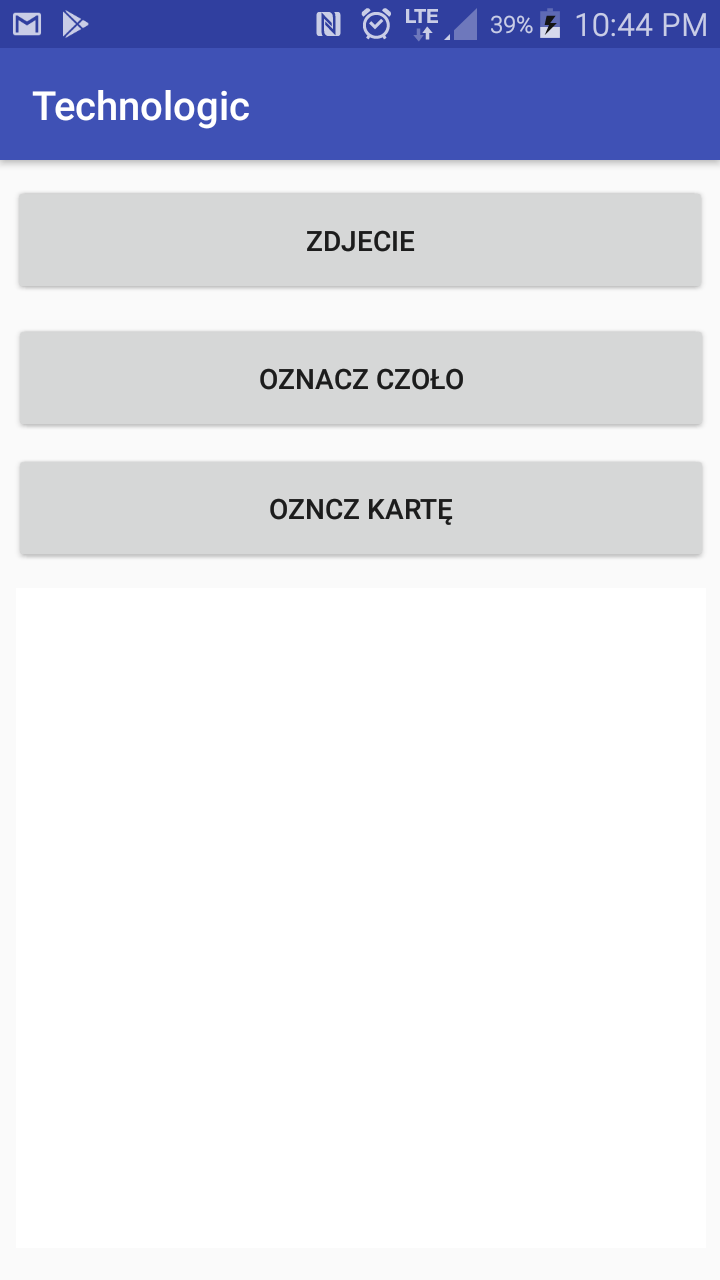
\includegraphics[width=\linewidth]{imgs/puste.png}
        \caption{po uruchomieniu}
        \label{fig:pustaAktywnosc}
    \end{subfigure}\hfill
    \begin{subfigure}{0.25\textwidth}
        \centering
        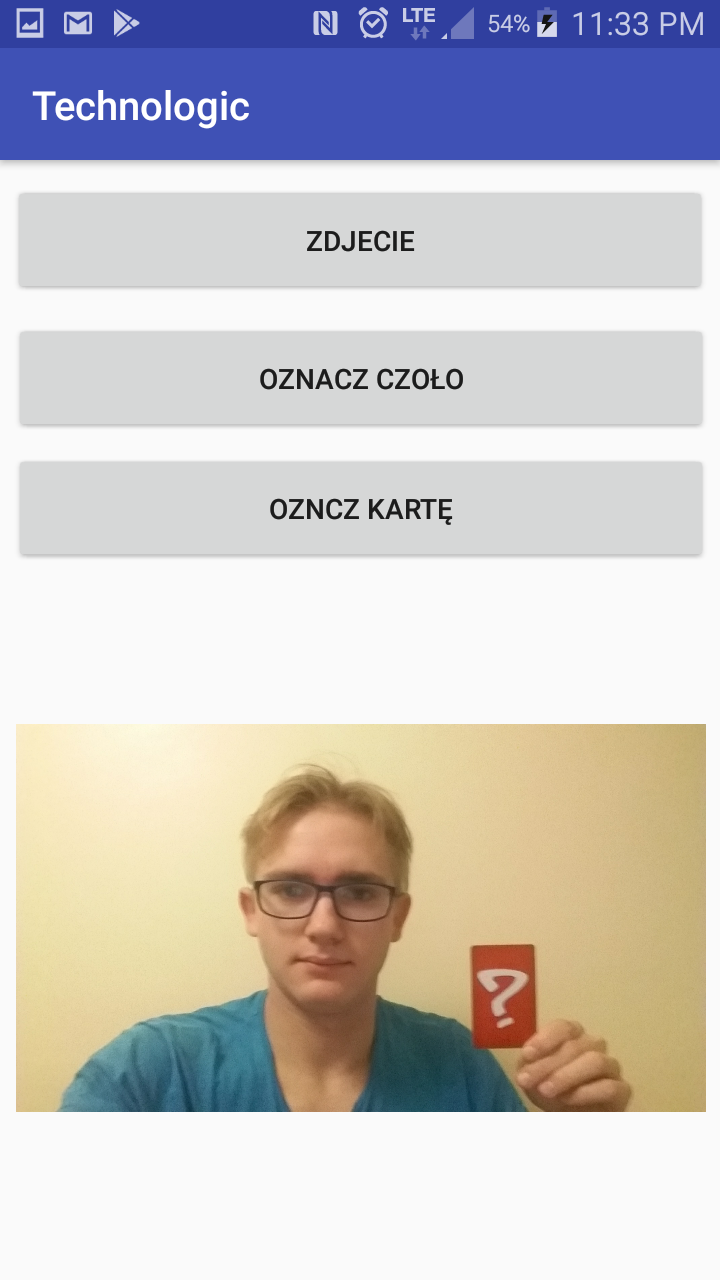
\includegraphics[width=\linewidth]{imgs/czyste.png}
        \caption{po wykonaniu zdjęcia}
        \label{fig:pusteZdjecie}
    \end{subfigure}\hfill
    \begin{subfigure}{0.25\textwidth}
        \centering
        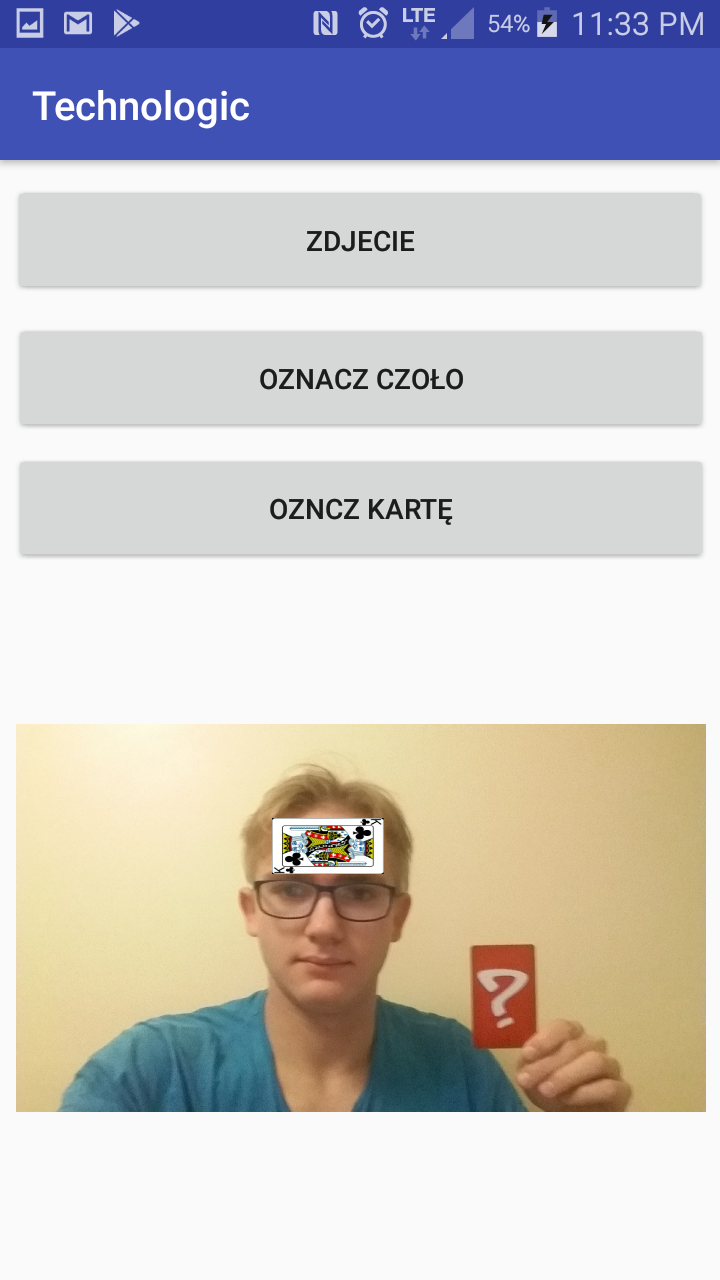
\includegraphics[width=\linewidth]{imgs/czolo.png}
        \caption{po detekcji czoła}
        \label{fig:zdjecieCzolo}
    \end{subfigure}\hfill
    \begin{subfigure}{0.25\textwidth}
        \centering
        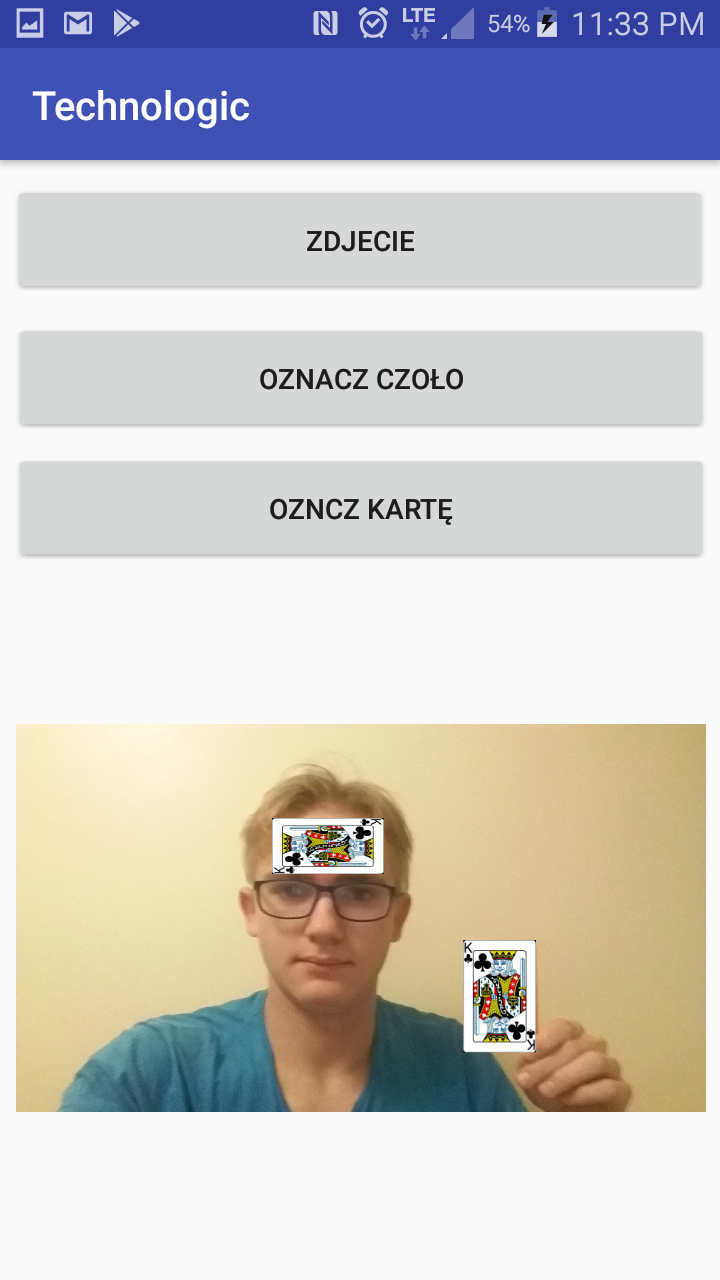
\includegraphics[width=\linewidth]{imgs/oba.png}
        \caption{po detekcji karty}
        \label{fig:zdjecieObo}
    \end{subfigure}
    \caption{Widoki aktywności obsługującej zdjęcia}
    \label{widokiPhoto}
\end{figure}

Rysunek \ref{widokiPhoto} przedstawia widok Aktywności w której realizowane są operacje związane ze zdjęciem. Widok aktywności składa się z trzech przycisków oraz okienka z obrazkiem. 
Po wciśnięciu przycisku z napisem ZDJĘCIE zostaje uruchomiona systemowa aplikacja aparatu, która po wykonaniu zdjęcia prosi o zatwierdzenie wykonanego zdjęcia. Jeśli zaakceptowano zdjęcie następuje automatyczny powrót do naszej aplikacji.
Po stronie naszej aplikacji kod wygląda następująco:

\begin{lstlisting}[language=Java]
public void takePic(){
    pictureFile = getPictureFile();
    Intent intent = new Intent(MediaStore.ACTION_IMAGE_CAPTURE);
    intent.putExtra(MediaStore.EXTRA_OUTPUT, Uri.fromFile(getPictureFile()));
    //pathPic = dest.getPath();        ((Activity)mainContext).startActivityForResult(intent, REQUEST_IMAGE);
}
@Override
protected void onActivityResult(int requestCode, int resultCode, Intent data) {
    if( requestCode == pictureService.REQUEST_IMAGE && resultCode == Activity.RESULT_OK ){
        pictureService.updateImage();
    }
}
\end{lstlisting}

Po wykonaniu zdjęcia w okienku pojawia się wykonane zdjęcie tak jak na rysunku \ref{fig:pusteZdjecie}. Następnie w zależności od wariantu sztuczki można wybrać przycisk OZNACZ CZOŁO albo OZNACZ KARTĘ. W przypadku pierwszego uruchamiamy następującą funkcję, która naniesie obraz karty w miejsce odnalezienia czoła:

\begin{lstlisting}[language=Java]
public Mat picToMark(Mat aInputFrame) throws IOException {
    Imgproc.cvtColor(aInputFrame, grayscaleImage, Imgproc.COLOR_RGBA2RGB);
    ObjectReconizer fR=new ObjectReconizer(mainContext, R.raw.lbpcascade_frontalface, mainContext.getString(R.string.cascadeFrontalFaceXML), grayscaleImage, 1.3, 3);
    MatOfRect faces=fR.getObjects();
    org.opencv.core.Rect[] facesArray = faces.toArray();
    if(facesArray.length>0) {
        ObjectReconizer eR=new ObjectReconizer(mainContext, R.raw.haarcascade_lefteye_2splits, "haarcascade_lefteye_2splits.xml", grayscaleImage, 1.3, 3);
        for (int i = 0; i < facesArray.length; i++) {
            org.opencv.core.Rect face=facesArray[i];
            org.opencv.core.Rect abcd =new org.opencv.core.Rect(face.x, face.y, face.width, face.height);
            Mat roi_color= new Mat(aInputFrame, abcd);
            eR.setGrayScaleImage(roi_color);
            MatOfRect eyes=eR.getObjects();
            org.opencv.core.Rect[] eyesArray=eyes.toArray();
            if(eyesArray.length==2){
                int x=(eyesArray[0].x<eyesArray[1].x) ? eyesArray[0].x:eyesArray[1].x;
                int x2=(eyesArray[0].x>eyesArray[1].x) ? eyesArray[0].x+eyesArray[0].width:eyesArray[1].x+eyesArray[1].width;
                int y = eyesArray[0].y;
                int w=x2-x;
                int h=w/2;
                insertCardIntoImage(roi_color, new Point(0, x), new Point(h, w+x));
            }
        }
    }
    return aInputFrame;
}
\end{lstlisting}

Po wykonaniu tej operacji w miejsce odnalezienia czoła zostanie wklejony obraz karty, tak jak na rysunku \ref{fig:zdjecieCzolo}. 
Jeśli wybrany jest wariant by karta została wklejona w miejsce naszego znaku zapytania wybieramy przycisk OZNACZ KARTĘ w tym wypadku uruchomi się następująca funkcja:

\begin{lstlisting}[language=Java]
public void markCard() throws IOException {
    if(grayscaleImage==null)grayscaleImage=new Mat();
    Mat pictureToMark= Imgcodecs.imread(pictureFile.getPath());
    double width=pictureToMark.size().width;
    double height=pictureToMark.size().height;
    MatOfRect cards = new MatOfRect();
    while(width>120.0){
        Imgproc.cvtColor(pictureToMark, grayscaleImage, Imgproc.COLOR_RGBA2RGB);
        ObjectReconizer cR=new ObjectReconizer(mainContext, R.raw.newcard, "newcard.xml", grayscaleImage, 1.4, 25);
        cards=cR.getObjects();
        if(cards.toArray().length!=1){
            width/=1.5;
            height/=1.5;
            Imgproc.resize(pictureToMark, pictureToMark, new Size(width,height ));
        }
        else break;
    }
    org.opencv.core.Rect[] cardsArray = cards.toArray();
    if(cardsArray.length==1){
        Mat picToMarkAfterResize = Imgcodecs.imread(pictureFile.getPath());
        double ratio= picToMarkAfterResize.size().width/width;
        Point lt=new Point(cardsArray[0].tl().x*ratio, cardsArray[0].tl().y*ratio);
        Point br=new Point(cardsArray[0].br().x*ratio, cardsArray[0].br().y*ratio);
        insertCardIntoImage(picToMarkAfterResize, lt, br);
        pictureToMark=picToMarkAfterResize;
    }
    pictureFile = getPictureFile();
    Imgcodecs.imwrite(pictureFile.getPath(), pictureToMark);
    updateImage();
}
\end{lstlisting}

Po wykonaniu tej operacji karta została wklejona w miejsce odnalezionego obiektu. Rysunek \ref{fig:zdjecieObo} przedstawia widok po wykonaniu detekcji karty po wcześniejszej detekcji czoła.
